\documentclass{FastFyp}

\begin{document}
\newcommand{\supervisor}{Dr. Mirza Mubasher Baig}
\newcommand{\university}{National University of Computer and Emerging Sciences, Lahore}
\newcommand{\fyptitle}{NextGenYield}
\newcommand{\degree}{BS}
\newcommand{\Studentone}{Shawaiz Ali Rehman     23L-0510    BS(CS)} 
\newcommand{\Studenttwo}{Aimen Abdul Rehman     23L-0670    BS(CS)}
\newcommand{\Studentthree}{Hassan Khan     23L-0800    BS(CS)}
\date{\today}
\renewcommand{\contentsname}{Table of Contents}

\makeatletter
    \begin{titlepage}
        
\includegraphics[width=0.2\linewidth]{Figures/nulogo.png}\hfill
        
\includegraphics[width=0.2\linewidth]{Figures/fast.png}\\
        \begin{center} 
            {\large\bfseries \university}\\[7ex]
            
\includegraphics[width=0.4\linewidth]{Figures/fastlogo.png}\\[8ex]
            {\huge \bfseries  \fyptitle }\\[10ex] 
            {\Studentone}\\{\Studenttwo}\\{\Studentthree}\\[4ex] 
            {Supervisor: \supervisor} \\ [10ex]
            {Final Year Project}\\
            {\large \@date}
        \end{center}
    \end{titlepage}    
\makeatother
\frontmatter

\newpage \thispagestyle{empty} \mbox{} \newpage %Aatira

\pagestyle{empty}  %Aatira
\section*{\begin{center}{Anti-Plagiarism Declaration} \end{center}} %Aatira
This is to declare that the above publication was produced under the:
\begin{flushleft}
\bf Title: \fyptitle
\end{flushleft}

is the sole contribution of the author(s), and no part hereof has been reproduced as it is the basis (cut and paste) that can be considered Plagiarism. All referenced parts have been used to argue the idea and cited properly. I/We will be responsible and liable for any consequence if a violation of this declaration is determined.
\\[4ex]
%% FYPTODO add the date and your names here
Date: ..........................

\begin{flushright}
Name: ..........................
\\[3ex]
Signature: ..........................
\\[6ex]
Name: ..........................
\\[3ex]
Signature: ..........................
\\[6ex]
Name: ..........................
\\[3ex]
Signature: ..........................

\end{flushright} 

\vspace{5 cm} %Aatira
 
\hrule %Aatira

\section*{Author's Declaration}
This states Authors’ declaration that the work presented in the report is their own, and has not been submitted/presented previously to any other institution or organization.
\pagebreak
\section*{Abstract}
Well-timed detection of crop developmental stages is essential for improving agriculture management practices and reducing potential yield losses. This study proposes an intelligent crop monitoring system and decision support system utilizing the FoMO4Wheat agriculture, a self supervised model trained on extensive wheat imagery. A classification layer is added to the frozen transformer features  to divide wheat canopy imagery into six key growth stages, from tillering to complete growth. These sequential observations are recorded into a temporal growth timeline, which is then used by a rule-based argonomic system to provide guidance on scheduling , nutrient application, and possible crop risks. By combining visual crop analysis with practical farming recommendations , the proposed system provides an easy to use , data driven tool for precision crop management. 
\pagebreak 

\section*{Executive Summary}
The executive summary should be one to two pages’ of an overview of the information contained in the FYP report.  It should give the reader an easy reference, in a very brief form, to the important information contained in the report and explained in more detail in the body of the report. People reading the report will use this section as a reference during presentations. 
\pagebreak


\pagestyle{fancy} %Aatira
\tableofcontents

\pagebreak
\listoffigures	% comment this if there are no figures
\addcontentsline{toc}{chapter}{List of Figures}
\pagebreak
\listoftables % comment this if there are no tables
\addcontentsline{toc}{chapter}{List of Tables}

\mainmatter


\chapter{Introduction}
In traditional farming wheat production depends upon visual observation and fixed schedule dates. However, field decisions require knowing the exact growth stage of the crop, which does not always follow a calendar. These methods may not consider changes in the temperature ,weather and the growth of crops which can have farmers giving wrong inputs at the wrong time ,this results in wasting the resources and reduces crop production.

To solve this problem, this project develops an intelligent crop monitoring system which is NextGenYield. It is based on FoMo4Wheat, a vision model trained on nearly 2.5 million wheat canopy pictures. This system identifies 6 important wheat growth stages using a classification layer. The photos are smartphone photos. It also tracks the growth of the crop and gives farmers simple recommendations for fertilizing and usage of water percentage at the right time with preventing crop hazards.

 
\section{Purpose of this Document}

The main purpose of this document is to give the details of the development and evaluation of our Final year project, NextGenYield. The document mentions the technological methodology,data pipeline, and field validation needed to turn advanced computer vision models into a reliable smartphone app for farmers. The document answers the question: 

\textbf{Can a wheat vision model which is trained using research images , accurately detect the wheat growth stages from ordinary photos taken in real farm condition?}

Also it takes into consideration whether adding a simple classification layer can improve the model and allow it to be more useful in terms of giving useful recommendations to farmers. This report includes the completion of the system, its methods ,architecture, testing ,implementation ,limitations and testing with the possible improvement of the future work.

 
\section{Intended Audience}
The main audience for this report are the panel reviewing this FYP, agriculture experts interested in crop monitoring and tech developers working on mobile apps for farmers and researchers interested in using image based models to study the crop growth. 

\section{Definitions, Acronyms, and Abbreviations}

\textbf{FYP}: Final Year Project  

\textbf{AI}: Artificial Intelligence  

\textbf{ML}: Machine Learning  

\textbf{DL}: Deep Learning  

\textbf{ViT}: Vision Transformer  

\textbf{FoMo4Wheat}: Foundation Model for Wheat  

\textbf{WGSP}: Wheat Growth Stage Prediction  

\textbf{API}: Application Programming Interface  

\textbf{REST}: Representational State Transfer  

\textbf{UI}: User Interface  

\textbf{UX}: User Experience  

\textbf{MVP}: Minimum Viable Product

 
\section{Conclusion}
In Conclusion, ”NextGenYeild” is ready to transform precision agriculture by fusing a user-friendly mobile interface with a reliable AI-driven back-end system. In addition to streamlining crop monitoring for farmers, the platform makes use of cutting-edge technology like the FoMo4Wheat vision foundation model and downstream phenological classification to improve user experience and guarantee data validity. The team is dedicated to creating a platform that strikes a balance between computational accuracy and real-world field usability, ensuring that every stakeholder benefits from its services. This will be accomplished through thorough experimental evaluation on local field imagery and by grounding all decision-support in established agronomic principles.

(Note: This conclusion paragraph is a placeholder and will be updated to reflect the full chapter-by-chapter report outline once all subsequent chapters are finalized).

 
\chapter{Project Vision}
Traditional farmers check their crops by checking them manually and with fixed date schedules. But due to the recent inventions in AI and computer vision has provided us with new ways to make farming easy and smarter. Our project aims to use these technologies to make a smart and much more intelligent crop monitoring system.This system will provide us with a strong foundation which can later be used to support different crops and various useful decision making for farmers. The aim of this chapter is to address the agriculture problems. 
\section{Problem Domain Overview}
Wheat is the most needed and powerful crop in the world.it is a part of a major source of calories and protein for people all around the world. Therefore, wheat farming is very important for farming countries. During its growth it passes through several stages like stem elongation,booting and tillering. Each stage is in different needs of soil,water and nutrients. Changes in weather,seed and temperature affect the growth rate of wheat. And due to this farmers cannot rely on fixed dates to determine the stage of wheat. Therefore, regular monitoring is very important for the production of the yield crop. 
\section{Problem Statement}
Improving farming practices for wheat yield needs sufficient water, fertilizer, and necessary treatment at accurate biological growth stages. However, farmers conventionally rely on visual checks or fixed calendar days, which results in growth variations due to weather and often leads to resource waste and less crop growth. Furthermore, existing solutions lack advance vision capabilities , unable to track temporal over time, reliable and evidence based guidance.  

\section{Problem Elaboration}
Smart crop monitoring only works in real fields if one big farming problem and a few technical ones are solved. The main problem is that farmers give water and fertilizers at the wrong time because they cannot detect the growth stage of the wheat. On the technical side, phone cameras struggle outdoors because sunlight changes through the day, pictures are taken at awkward angles, and the soil in the background is cluttered, so older CNN models get confused. Stages that come one after another also look almost the same, and separating them requires noticing more than 700 tiny details of plant form that standard vision models cannot catch. There is also very little labeled phone imagery from real local farms, so models have too few examples to train on. Finally, existing tools judge each picture by itself and do not keep a record of growth over time, which means they cannot tell farmers when to irrigate, fertilize, or protect their crops. 
\section{Goals and Objectives}
Write goals and objectives here.
\section{Project Scope}
The scope of this project is a mobile application for wheat farmers,which monitors the growth stages of the crop and gives timely suggestions and decision support. 

The application will allow farmers to:
\begin{itemize}
    \item Take wheat canopy images and upload to the app using ordinary camera of the smartphone
    \item Classify the six important stages of wheat's growth which includes stages of (tillering, jointing, booting, anthesis, grain filling, and maturity)
    \item Visualise and track growth timelines for each field across the chronological observations.
    \item Receive rule-based and deterministic suggestions for irrigation timing, fertilizer scheduling, and hazard prevention.
\end{itemize}
 For the Ai inference pipeline Python and PyTorch will be used. A pretrained vision model will be used as a foundation and a special layer for classification will be trained on top of it. This will be combined with a mobile framework such as React Native or Flutter for the frontend. The application will use REST API to communicate with the backend. Agile development principles will be used while developing the project and management of the project will be done iteratively.
 
 The project deliverables will include:

\begin{itemize}
    \item A functional mobile application and backend service for wheat growth-stage monitoring and farmer decision support
    \item A trained and validated downstream classification pipeline evaluated on realistic field imagery
    \item Comprehensive documentation of the design, implementation, and experimental testing process
\end{itemize}

 The project scope does not include the following: 
 
\begin{itemize}
    \item Utilising of autonomous drone or automated robotic hardware
    \item Estimating direct crop yield in absolute quantities (such as kilograms per hectare)
    \item Using Large Language Models to suggest unverified chemical dosage
    \item Use, deployment and maintenance of IoT sensors network.
\end{itemize}

\section{Sustainable Development Goal (SDG)}
NextGenYeild demonstrates how the platform contributes to sustainable agriculture as it improves crop productivity and helps in reliable food production. Ultimately, the project’s goal is to strengthen harvest resilience and promote food security by helping ensure access to healthy and fresh food.  
\newline
\begin{figure} [!h]
    \centering
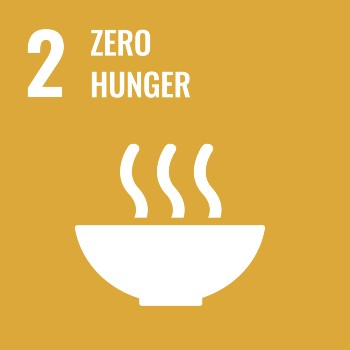
\includegraphics[width=0.4\textwidth]{Figures/sdg2.jpg}
    \caption{\textbf{Sustainable Development Goal} }
    \label{fig:1}
    This figure represents our sustainable development goal which is Zero Hunger
\end{figure}
\section{Constraints}
The following are the main constraints of the system’s design and implementation:

\begin{itemize}
    \item \textbf{Functional Scope:} The image will strictly limit the functional scope to wheat growth staging with timeline tracking and decision support. No physical drones / IoT hardware nor direct yield forecasting.
    \item \textbf{Compute Resources:} Model adaptation and inference are limited to one of the local workstations of a member which has an Rtx 5070 Graphics card.
    \item \textbf{Timeline: }Each phase of development, testing and documentation must happen within 2 semesters (9-12 months). 
    \item \textbf{Team Allocation:} In a group of three members, Engineering tasks, model experimentation and UI design are done in the project.
    \item \textbf{Advisory Integrity: }Recommendations should be given based on deterministic agronomic rules that are verified and validated. They must not come from a text generation model. AI techniques such as LLM or numerical AI can give wrong recommendations.
    \item \textbf{Accessibility: }The app should be lightweight , intuitive, and easily operable for farmers.
\end{itemize}

 
\section{Business Opportunity}
The potential for the app to commercially become a standalone business in the precision agriculture sector is very high. The business model can adopt a freemium approach providing basic growth-stage tracking for free while monetizing individual farmers by charging them their subscription fee for premium features. The premium features will include advanced timeline tracking, risk alerts, customised irrigation and fertiliser schedules specific to each field of a farmer.
NextGen Yield can also be licensed as an enterprise B2B software or an API which can be used by agriculture corporations, fertilizer companies, and crop insurance firms. Through periodic visits and photographs, the organisation can monitor large areas of farmland that they have contracted. 

 
\section{Stakeholders Description/ User Characteristics}
Identify and briefly describe who the users of this system will be, and their roles.
\subsection{Stakeholders Summary}
\subsection{Key High-Level Goals and Problems of Stakeholders}
Notice how a section’s heading is changed to “heading 1”.  It will show up in the table of contents as a section under a chapter.  Notice its numbering also. Similarly, subsections can have heading 2 and heading 3 styles.\\
\textcolor{red}{NOTE: Subsections from 2.7 to 2.9 are optional for Research projects but compulsory for Development projects.}

\chapter{Literature Review / Related Work}
This chapter reviews related work that is already existing on crop monitoring, wheat growth stage detection and agricultural decision support systems that are related to NextGenYield. The literature is grouped into categories for example image-based wheat growth stage recognition, satellite and remote crop monitoring, image based plant disease detection, AI generated agronomic advice. By reviewing these systems we analysed their methods, capabilities, and limitations, while also highlighting gaps that provide a foundation for developing NextGenYeild as a practical smartphone-based crop monitoring and decision-support system. 
\section{Definitions, Acronyms, and Abbreviations}
\textcolor{red}{To be entered when this chapter is completed} 
\section{Detailed Literature Review} 
In this section each related work is discussed in detail, moreover each work is critically analysed and explained how it relates or connects to NextGenYield.
\subsection{Category A: Image-Based Wheat Growth-Stage Recognition}

The studies in this category are closest to the core task of NextGenYield. They show that images can be used to detect growth stages of wheat but each of them depend on equipment, controlled conditions or sources of data that an ordinary farmer may not have access to.

\subsubsection{Near-Surface Camera Phenology with Spatiotemporal Fusion}

\textbf{Summary}

Cai et al. [1] developed a system that detects wheat growth stages by using fixed cameras. The system was at Baima Experimental Station of Nanjing Agricultural University in China. For 107 days a camera which was placed three metres above the ground took images from 8am to 5pm ,during the 2022-2022 growing season. The images were labeled into eight stages of growth ,from emergence to maturity. The researchers used ResNet50 as their base model and tried three different methods for combining spatial and chronological information . The best model was the one which combined an LSTM with ResNet50,and it achieved an accuracy of 93.5\%. The study also found that results can be improved by taking higher resolution images, positioning the camera at about 40-60 degrees and fine tuning in two steps.

\textbf{Critical Analysis of the Research Item}

A strength of this study is that it carefully analyses design factors and confusion matrices that tell which stages are hard. The sequential model was weakest at anthesis. The finding that camera angle affects accuracy is useful for setting standard methods to capture image. However there are some practical limitations. The data was collected in one location only and in one growing season , moreover a fixed camera at a set height was used. Moreover the model required a sequence of 30 images instead of using one image. Since the series of images came from the same plots (6 total)and then split randomly, so performance was not demonstrated on an unseen field. The large model size also may need to be reduced for realtime use.

\textbf{Relationship to the Proposed Research Work}

nextGenYield handles the same task but it doesn't use installed cameras. Instead a farmer takes an image straight from his smartphone at irregular intervals, the classifier works on that single image, and the chronological reasoning and decisions are made within the app later on without any use of a neural network. The camera viewing angle technique helps us give farmers a guideline in the app of how to capture the image for best results.

\subsubsection{GSP-AI: Growth Stage Prediction from Drone Images and Climate Data}

\textbf{Summary}

Shen et al. [2] developed GSP-AI. It is a deep-learning platform that uses drone images and weather  data to classify important wheat growth stages and predict flowering time. To train the modal they also created the Wheat Growth Stage Prediction (WGSP) dataset, which contains 70,410 labelled images from different wheat varieties in China, the United Kingdom, and the United States, along with related climate data. The study aims to help breeders and researchers in monitoring the growth stages of large numbers of varieties of wheat in different locations and different seasons.

\textbf{Critical Analysis of the Research Item}

The main strength is the dataset, it is large,consists of images of multiple countries, is openly available and is labelled by growth stage. This makes it a useful dataset for future. Combining images with climate data is also a good way to improve flowering-time prediction. However from a farmer’s point of view there are some limitations. The system depends on drone flights and drone flights can be affected by rain[1].The model is designed for breeding research rather than helping farmers make decisions such as when to irrigate , fertilise etc. The paper also does not provide any system that advises the farmer.\\


\textbf{Relationship to the Proposed Research Work}

WGSP provides the six-stage taxonomy and the dataset against which the NextGenYield classification head can be trained and/or evaluated. NextGenYield replaces drone imagery with smartphone photographs and for the classification step it does not require weather information. Moreover NextGenYield adds the missing layers absent in the study,which are a growth timeline and stage-specific advice.

\subsubsection{DenseNet--BiLSTM Growth-Stage Determination from Image Sequences}

\textbf{Summary}

Wang et al. [3] studied wheat growth-stage recognition . They growed wheat in a controlled climate room. Four different varieties of wheat were photographed every week from eighth fixed camera angles.The temperature of the room was kept at 23 °C with light for 16 hours and dark for 8 hoursand 90\% humidity. The researchers removed the background using K-means colour clustering and used DenseNet201 model with a bidirectional LSTM to identify the five growth stages: tillering, re-greening, jointing, booting, and heading. The model achieved an accuracy of 98.43\% on 40 test sequences.They performed better than basic CNN and CNN--LSTM models.

\textbf{Critical Analysis of the Research Item}

The study shows that results can be improved in detecting the growth stages if we use a sequence of images instead of a single image. However, the dataset is small, 592 sequences and 3483 images. The data is also unbalanced, with only 72 images showing the booting stage and only 7 of these in the test set. Booting had the lowest precision at 85.71\% meaning the overall accuracy is a result of the outputs of the common stages. The authors also state that they faced problems in changing the lights, having parts of plants blocked, and addressing real field conditions before the system can be used in actual fields.

\textbf{Relationship to the Proposed Research Work}

This work is an example of why NextGenYield will report the metrics for each stage rather than one aggregate accuracy. It also highlights the gaps that NextGenYield aims to address by working with real field images that contain soil, shadows, nearby plants,weeds and an image that is not taken at a fixed angle or with a professional camera. 
\section{Literature Review Summary Table}
The related work summary table is shown in \ref{tab:1}
\begin{table}[!h]
\centering
\caption{\textbf{Related Work Review Summary Table} }\textit{This summary table lists the eight works discussed throughout this chapter.}
\newline

\begin{tabular}{|p{2.5cm}|p{2.5cm}|p{4cm}|p{5cm}|}
\hline
    \textbf{Application} & \textbf{Features} & \textbf{Relevance} & \textbf{Limitations} \\
\hline
Cai et al. \cite{ref:Cai:2024} & Fixed-camera image series; CNN--LSTM fusion; eight stages & Shows camera angle and resolution affect stage accuracy & One station and one season; needs image series and fixed cameras; heavy model \\
\hline
GSP-AI \cite{ref:Shen:2024} & Drone images plus climate data; WGSP dataset of 70,410 images & Source of the six-stage taxonomy and benchmark & Needs drone flights and weather records; built for breeding plots \\
\hline
Wang et al. \cite{ref:Wang:2025} & DenseNet--BiLSTM on growth-chamber image sequences & Shows why per-class results matter (booting weakest) & Controlled environment; five stages; only 72 booting images \\
\hline
Bhatti et al. \cite{ref:Bhatti:2024} & Sentinel-2 NDVI compared with daily field cameras, Sargodha, Punjab & Local evidence on the limits of satellite monitoring & Fog and cloud gaps; lower NDVI than cameras; no discrete stage labels \\
\hline
Mohanty et al. \cite{ref:Mohanty:2016} & CNN on 54,306 PlantVillage leaf images & Illustrates the lab-to-field accuracy gap & 99.35\% on lab test set but 31.4\% on images from other sources \\
\hline
Plantix \cite{ref:CABI:2020} & Photo diagnosis of about 400 pests, diseases and deficiencies; treatment tips & Closest farmer-facing app, but disease-focused & Modest initial accuracy in independent test; no growth-stage tracking \\
\hline
Ibrahim et al. \cite{ref:Ibrahim:2024} & ChatGPT compared with extension agents on Nigerian rice questions & Evidence against free-text advice on rates and timing & Weak on planting time and fertiliser rate and timing; small sample \\
\hline
FoMo4Wheat \cite{ref:Han:2025} & ViT foundation model pretrained on 2.5 million wheat images & Backbone used by NextGenYield & Heavy for edge devices; wheat-focused; not trained on phone photos \\
\hline
\end{tabular}
\label{tab:1}
\end{table}


\section{Conclusion}
Write the conclusion of the literature review. 
The columns in the table depending upon your problem and should be specific to your project as described in \ref{tab:1}, \ref{tab:2}, respectively. Proper citations and references are necessary. The template has already an integrated IEEE references format. Go to Google scholar, copy the bib text of your reference, and paste the reference into the fypbib.bib file. Then all you have to do is use \cite{ref:Bishop:2006}.\\ \textcolor{red}{\textbf{NOTE: For development projects, describe related or similar work done by other teams and details of their methods/algorithms. For a research project, a detailed literature survey is expected.}}
 
\chapter{Software Requirement Specifications}
This chapter provides a comprehensive and detailed specification of the software requirements for \textbf{NextGenYield: Wheat Crop Decision Support and Vision AI System}. It delineates the functional and non-functional requirements, defines quality attributes, hardware and software runtime constraints, user-interaction use cases, graphical user interface architecture, database entity-relationship models, data dictionaries, and an exhaustive risk analysis. The objective of this specification is to furnish an unambiguous engineering blueprint that enables researchers, software engineers, and agricultural domain specialists to understand, verify, and reproduce the entire software system.

\section{List of Features}
NextGenYield provides a mobile-first, AI-driven precision agriculture ecosystem tailored specifically for wheat smallholder farmers, landowners, agronomic professionals, and input manufacturers. The primary features of the system include:

\begin{enumerate}
    \item \textbf{Foundation Model-Powered Phenological Classification:} Utilizes the specialized \textit{FoMo4Wheat} Vision Transformer (ViT-B/14, 86.6M parameters) pre-trained on 2.5 million agricultural images. A downstream classification head classifies crop canopy imagery into six distinct biological growth stages (Tillering, Jointing, Booting, Flowering, Grain Filling, and Maturity) without requiring extensive computational resources on the client side.
    \item \textbf{Real-Time Edge Image Quality and Angle Compliance Guardrail:} An onboard sensor-fusion filter running on the smartphone's client layer that leverages the hardware gyroscope, accelerometer, and Laplacian edge-variance computation. It prevents degraded or non-compliant field photography by actively guiding farmers into capturing oblique-to-downward canopy imagery ($45^\circ - 80^\circ$ tilt) with adequate sharpness before image transmission.
    \item \textbf{Decoupled Field Demarcation and GeoJSON Boundary Creation:} An interactive GIS mapping tool allowing farmers and landowners to demarcate field parcel perimeters directly upon high-resolution satellite and cadastral map overlays. It provides four distinct boundary geometries---Square, Rectangle, Polygon (multi-vertex), and Circle (centre-pivot radial)---generating standardized RFC 7946 GeoJSON representations with real-time acreage and square-meter calculations.
    \item \textbf{Decoupled Crop Cycle Initialization:} Land parcel boundary creation is strictly separated from agricultural crop inputs. Once a field boundary is established, farmers initiate a 140-day crop cycle only when the land is prepared for sowing, entering seed variety (e.g., Akbar-2019, Dilkash-20), certified seed source, fertilizer manufacturer (FFC, Engro, Fatima), and sowing date exactly once.
    \item \textbf{Deterministic, Hallucination-Free Agronomic Advisory Engine:} Eliminates probabilistic Large Language Model (LLM) text hallucinations by employing a rule-governed agronomic knowledge base. Crop growth stage transitions are deterministically mapped to verified provincial agricultural protocols, generating stage-specific irrigation schedules, fertilizer split dosages, and disease warnings (e.g., yellow stripe rust prevention during booting).
    \item \textbf{Temporal Crop Growth Timeline Engine:} Maintains a persistent, timestamped chronological ledger of all visual observations, stage confidence scores, and photographic records per field. It tracks cumulative Days After Sowing (DAS) and computes phenological velocity to detect delayed germination or premature senescence.
    \item \textbf{Collective Farm Intelligence and Regional GIS Mapping:} Provides a spatial visualization of neighboring wheat parcels across the agricultural district (e.g., Faisalabad division). Fields are color-coded by current phenological stage, enabling peer observation, regional water management coordination along canal waterways, and disease spread monitoring.
    \item \textbf{Peer Benchmarking and Proven Techniques Showcase:} A collaborative peer showcase displaying verified top-yielding plots (54--62 Maunds/Acre). Farmers can inspect the complete 140-day crop cycle---including exact watering dates, weed filtering applications, fertilizer split timings, and seed variants---and adopt proven schedules directly into their own field calendar.
    \item \textbf{Farmer Accessibility, Bilingual Localization, and Audio Narration:} Engineered specifically for varying levels of digital and textual literacy. The interface offers full Urdu and English bilingual toggles, high-contrast light mode optimized for harsh direct field sunlight, adjustable typography scaling, and integrated audio synthesis that reads agronomic advisories aloud in spoken Urdu.
\end{enumerate}

\section{Functional Requirements}
The functional requirements specify the operational capabilities and behaviors that NextGenYield must support for its primary actors: Farmers/Landowners, Agricultural Stakeholders, and the Underlying System.

\subsection{Functional Requirements for Farmers and Landowners}
Farmers and landowners using the mobile application shall be able to:
\begin{enumerate}
    \item \textbf{Account Registration and Profile Authentication:} Create a user profile using phone number authentication or credentials, storing personal details, primary village/district location, and language preference.
    \item \textbf{Demarcate Land Boundaries on GIS Map:} Add and delineate farm parcels using interactive map boundary tools (Square, Rectangle, Multi-Vertex Polygon, and Centre-Pivot Circle) over satellite or cadastral views.
    \item \textbf{Inspect Calculated Area in Real Time:} View automatically calculated parcel measurements in both standard agricultural Acres and metric square meters ($\text{m}^2$).
    \item \textbf{Initiate Crop Cycle:} Activate an unstarted (fallow) field parcel by entering the wheat seed cultivar, certified seed supplier, fertilizer manufacturing brand, sowing technique, and sowing date.
    \item \textbf{Execute Sensor-Guided Field Photography:} Capture canopy imagery using a camera interface equipped with real-time pitch angle reticles ($45^\circ - 80^\circ$ compliance) and Laplacian blur detection.
    \item \textbf{Receive Automated Growth Stage Classification:} Obtain instant phenological identification across six wheat growth stages accompanied by an AI classification confidence score.
    \item \textbf{Access Actionable Agronomic Guidance:} Retrieve deterministic recommendations detailing immediate irrigation requirements, fertilizer split quantities per acre, and active pathogen hazards.
    \item \textbf{Listen to Spoken Advisory Narration:} Trigger text-to-speech audio guidance in spoken Urdu to comprehend recommendations without reading text on screen.
    \item \textbf{Review Chronological Field Timeline:} Inspect sequential photographic and stage observations logged since sowing date to evaluate crop development pace.
    \item \textbf{Explore Regional GIS Map:} View surrounding agricultural plots color-coded by growth stage and inspect public cadastral and agronomic attributes of neighboring fields.
    \item \textbf{Adopt Best-Practice Crop Schedules:} Browse top-performing benchmark yields, examine full 140-day crop management cycles, and replicate successful schedules into their own active fields.
\end{enumerate}

\subsection{Functional Requirements for Agricultural Stakeholders}
Agricultural extension officers, agronomic researchers, and fertilizer technical representatives shall be able to:
\begin{enumerate}
    \item \textbf{Monitor Regional Phenological Trends:} Access aggregated geospatial analytics illustrating district-wide stage distributions (e.g., percentage of fields in Jointing vs. Booting).
    \item \textbf{Audit Verified Harvest Yields:} Verify and record final weighbridge harvest yields (Maunds/Acre) for benchmark fields to maintain showcase integrity.
    \item \textbf{Update Deterministic Agronomic Protocols:} Modify stage-dependent threshold parameters, fertilizer dosing recommendations, and fungicide alerts according to updated agricultural research directives.
    \item \textbf{Assess Input Performance Analytics:} Evaluate comparative cultivar performance and fertilizer brand efficacy across varying soil textures (e.g., Sandy Loam vs. Clay Loam).
\end{enumerate}

\subsection{Functional Requirements of the NextGenYield System}
The core NextGenYield system shall be capable of:
\begin{enumerate}
    \item \textbf{Edge Sensor Fusion and Guardrail Verification:} Continuously evaluate hardware orientation vectors and compute frame variance to reject blurry or improperly oriented photographs prior to server upload.
    \item \textbf{Vision Foundation Model Inference:} Resize input canopy images to $518 \times 518$ resolution, execute forward-pass feature extraction across frozen ViT-B/14 transformer layers, and evaluate linear classification logits.
    \item \textbf{Geospatial Coordinate Processing:} Validate, project, and store field polygon geometries compliant with RFC 7946 GeoJSON specifications, executing spatial containment queries for district-wide mapping.
    \item \textbf{Deterministic Rule-Engine Resolution:} Map current classified growth stage, cumulative days after sowing, and registered fertilizer manufacturer to deterministic advisory guidelines without generative model hallucination.
    \item \textbf{Temporal State Management:} Dynamically track active vs. fallow field states, calculate developmental velocity, and trigger critical milestone alerts.
    \item \textbf{Bilingual Data Serialization:} Serve internationalized string tables and synthesize Urdu audio strings for low-literacy accessibility.
\end{enumerate}

\section{Quality Attributes}
To guarantee operational viability across rural agricultural environments, NextGenYield satisfies the following quality attributes:
\begin{itemize}
    \item \textbf{Usability and Ergonomics:} The application interface utilizes high-contrast visual tokens, prominent icon-driven navigation, localized Urdu terminology, and single-tap audio narration, accommodating farmers with limited smartphone proficiency.
    \item \textbf{Reliability:} The system maintains high service availability during peak agricultural seasons (November wheat sowing through April harvest), ensuring advisory continuity.
    \item \textbf{Performance and Latency:} On-device edge guardrails provide instant angle feedback ($< 50\text{ ms}$), and end-to-end vision model inference executes within $1.8\text{ seconds}$ over standard $3\text{G}/4\text{G}$ cellular connections.
    \item \textbf{Agronomic Safety and Accuracy:} Deterministic rule matching prevents over-fertilization or premature watering, eliminating toxic agricultural hazards.
    \item \textbf{Modularity and Reusability:} Client-side view controllers, edge sensors, backend microservices, and GIS engines are strictly decoupled through well-defined REST API interfaces.
    \item \textbf{Scalability:} Stateless model inference containers and spatial database indexing support thousands of concurrent field queries during peak morning and evening farming hours.
\end{itemize}

\section{Non-Functional Requirements}

\subsection{Performance}
\begin{itemize}
    \item Edge-based sensor angle validation and blur computation must execute in real time on mobile hardware ($< 50\text{ ms}$ latency).
    \item AI growth stage inference through the backend vision service must complete within $2.0\text{ seconds}$ under a nominal $4\text{G}$ network connection.
    \item The backend REST API must sustain at least $500$ concurrent user requests without response degradation exceeding $1.5\text{ seconds}$.
    \item Regional GIS map rendering of 100 localized plot polygons must render within $1.2\text{ seconds}$ of viewport settlement.
\end{itemize}

\subsection{Reliability and Availability}
\begin{itemize}
    \item The system shall achieve an operational availability of at least $99.5\%$ throughout the 140-day wheat cultivation season.
    \item In the event of network disconnection, the mobile client must cache captured observations, field boundaries, and advisory cards locally, synchronizing automatically when connectivity resumes.
\end{itemize}

\subsection{Usability and Accessibility}
\begin{itemize}
    \item All user-facing screens must support instantaneous toggling between English and localized Urdu.
    \item High-contrast light mode styling must enforce a contrast ratio exceeding $4.5:1$ (WCAG AA standard) to preserve legibility under direct ambient field sunlight exceeding 50,000 lux.
    \item All key agronomic recommendations must feature an audible spoken Urdu audio narration button accessible via a single touch.
    \item Typography must support standard ($1.0\times$) and enlarged ($1.15\times$) font multiplication modes.
\end{itemize}

\subsection{Reusability and Maintainability}
\begin{itemize}
    \item The mobile application code base must follow a modular component architecture (under cross-platform frameworks such as React Native or Flutter), strictly isolating UI components, translation keys, state providers, and mock fixtures.
    \item The deterministic advisory logic must be maintained in structured configuration schemas rather than hardcoded conditional trees, permitting rapid agronomic parameter updates without recompiling client binaries.
\end{itemize}

\subsection{Security and Data Integrity}
\begin{itemize}
    \item All telemetric observations, user credentials, and spatial coordinates transmitted over the public network must be encrypted via Transport Layer Security (TLS 1.3).
    \item Field polygon definitions must enforce strict topological validation (no self-intersecting loops or degenerate nodes) before persisting to the spatial database.
\end{itemize}

\section{Assumptions}
\begin{itemize}
    \item \textbf{Hardware Availability:} The primary user possesses an Android or iOS smartphone equipped with a functional optical camera, accelerometer, gyroscope, and GNSS/GPS location services.
    \item \textbf{Cellular Connectivity:} While the client supports local caching for offline observation capture, periodic internet connectivity ($2\text{G}/3\text{G}/4\text{G}$ or Wi-Fi) is assumed for model inference synchronization and satellite basemap tile streaming.
    \item \textbf{Crop Scope:} The current operational scope of NextGenYield focuses exclusively on bread wheat (\textit{Triticum aestivum}) cultivated within irrigated sub-tropical agricultural regimes (e.g., Indus Basin plains).
    \item \textbf{Third-Party Basemaps:} Map rendering depends on standard OpenStreetMap or Mapbox satellite raster tile services for aerial spatial boundary visualization.
\end{itemize}

\section{Hardware and Software Requirements}

\subsection{Hardware Requirements}
\begin{itemize}
    \item \textbf{Development Workstation:}
    \begin{itemize}
        \item Multi-core processor (Intel Core i7/AMD Ryzen 7 or Apple Silicon M-series).
        \item 16 GB DDR4/DDR5 RAM.
        \item 50 GB free solid-state storage.
        \item Dedicated GPU (NVIDIA RTX 3060 or higher with 8 GB+ VRAM) for model fine-tuning and PyTorch inference benchmarking.
    \end{itemize}
    \item \textbf{Target Client Mobile Device:}
    \begin{itemize}
        \item Operating System: Android 10.0+ (API level 29+) or iOS 15.0+.
        \item Camera: Minimum 8.0-megapixel rear optical sensor with autofocus.
        \item Integrated Sensors: 3-axis accelerometer and 3-axis gyroscope.
        \item Minimum RAM: 2.0 GB.
        \item Network: $3\text{G}$, $4\text{G}$ LTE, or Wi-Fi radio.
    \end{itemize}
\end{itemize}

\subsection{Software Requirements}
\begin{itemize}
    \item \textbf{Mobile Client Runtime:} Modern cross-platform mobile application framework (React Native or Flutter) supporting native hardware sensor access (accelerometer, gyroscope, camera), reactive state management, and integrated GIS mapping canvas.
    \item \textbf{Programming Languages:} TypeScript / Dart (client-side mobile application), Python 3.10+ (backend vision API and deterministic advisory services).
    \item \textbf{AI/Vision Framework:} PyTorch 2.x, Hugging Face Transformers, TorchVision, FoMo4Wheat ViT-B/14 pre-trained model checkpoint.
    \item \textbf{Backend Web Services:} FastAPI / Python ASGI runtime, Uvicorn server, Pydantic data schemas.
    \item \textbf{Database Management System:} PostgreSQL 15+ equipped with PostGIS extension for spatial polygon geometries and JSONB support for temporal cycle logs.
    \item \textbf{Operating Systems:} Windows 11 / Linux (Ubuntu 22.04 LTS) for development, target deployment on Android and iOS.
\end{itemize}

\section{Use Cases}
NextGenYield's operational workflow is structured into nine core use cases that cover user authentication, land demarcation, cycle initialization, AI canopy phenotyping, advisory generation, timeline tracking, GIS exploration, and peer benchmark adoption. Each usecase table details the actor actions and corresponding system responses across standard and alternative execution paths.
\begin{table}[!ht]
\small
\centering
\caption{Use Case 1: User Registration}
\label{tab:uc1}
\begin{tabular}{|lllll|}
\hline
\multicolumn{2}{|l|}{\textbf{Name}} &
  \multicolumn{3}{p{10.2cm}|}{User Registration} \\ \hline
\multicolumn{2}{|l|}{\textbf{Actors}} &
  \multicolumn{3}{p{10.2cm}|}{Smallholder Farmer, Landowner, Agricultural Stakeholder} \\ \hline
\multicolumn{2}{|l|}{\textbf{Summary}} &
  \multicolumn{3}{p{10.2cm}|}{A new user creates an account within the NextGenYield platform to manage farm parcels and receive personalized crop advisories.} \\ \hline
\multicolumn{2}{|l|}{\textbf{Pre-Conditions}} &
  \multicolumn{3}{p{10.2cm}|}{The user has installed the NextGenYield application and possesses an active mobile telephone number.} \\ \hline
\multicolumn{2}{|l|}{\textbf{Post-Conditions}} &
  \multicolumn{3}{p{10.2cm}|}{A user profile is created in the database, and authentication tokens are securely saved to the device.} \\ \hline
\multicolumn{2}{|l|}{\textbf{\begin{tabular}[c]{@{}l@{}}Special\\ Requirements\end{tabular}}} &
  \multicolumn{3}{p{10.2cm}|}{The user interface must support clear Urdu and English text prompts with large touch targets.} \\ \hline
\multicolumn{5}{|c|}{\textbf{Basic Flow}} \\ \hline
\multicolumn{3}{|c|}{\textbf{Actor Action}} &
  \multicolumn{2}{c|}{\textbf{System Response}} \\ \hline
\multicolumn{1}{|p{0.8cm}|}{1} &
  \multicolumn{2}{p{6.0cm}|}{User launches the application and selects ``Create Account''.} &
  \multicolumn{1}{p{0.8cm}|}{2} &
  \multicolumn{1}{p{5.6cm}|}{The system displays the registration form.} \\ \hline
\multicolumn{1}{|p{0.8cm}|}{3} &
  \multicolumn{2}{p{6.0cm}|}{User enters full name, mobile number, district, and preferred language (Urdu or English).} &
  \multicolumn{1}{p{0.8cm}|}{4} &
  \multicolumn{1}{p{5.6cm}|}{System records input data and validates telephone format.} \\ \hline
\multicolumn{1}{|p{0.8cm}|}{5} &
  \multicolumn{2}{p{6.0cm}|}{User creates a secure PIN or password.} &
  \multicolumn{1}{p{0.8cm}|}{6} &
  \multicolumn{1}{p{5.6cm}|}{System verifies PIN strength and confirms credentials match.} \\ \hline
\multicolumn{1}{|p{0.8cm}|}{7} &
  \multicolumn{2}{p{6.0cm}|}{User submits the registration form.} &
  \multicolumn{1}{p{0.8cm}|}{8} &
  \multicolumn{1}{p{5.6cm}|}{System creates user record, stores session tokens, and navigates to the Farm Dashboard.} \\ \hline
\multicolumn{5}{|c|}{\textbf{Alternative Flow}} \\ \hline
\multicolumn{1}{|p{0.8cm}|}{3} &
  \multicolumn{2}{p{6.0cm}|}{User enters an already registered mobile number.} &
  \multicolumn{1}{p{0.8cm}|}{4-A} &
  \multicolumn{1}{p{5.6cm}|}{System responds with an error message: Phone number already registered, and redirects to Login.} \\ \hline
\multicolumn{1}{|p{0.8cm}|}{7} &
  \multicolumn{2}{p{6.0cm}|}{User submits registration form without internet connectivity.} &
  \multicolumn{1}{p{0.8cm}|}{8-A} &
  \multicolumn{1}{p{5.6cm}|}{System responds with network failure alert and prompts user to retry.} \\ \hline
\end{tabular}
\end{table}

% Use Cases (all tables sit under one generic use case heading)

\begin{table}[!ht]
\small
\centering
\caption{Use Case 1: User Registration}
\label{tab:uc1}
\begin{tabular}{|lllll|}
\hline
\multicolumn{2}{|l|}{\textbf{Name}} &
  \multicolumn{3}{p{10.2cm}|}{User Registration} \\ \hline
\multicolumn{2}{|l|}{\textbf{Actors}} &
  \multicolumn{3}{p{10.2cm}|}{Smallholder Farmer, Landowner, Agricultural Stakeholder} \\ \hline
\multicolumn{2}{|l|}{\textbf{Summary}} &
  \multicolumn{3}{p{10.2cm}|}{A new user creates an account within the NextGenYield platform to manage farm parcels and receive personalized crop advisories.} \\ \hline
\multicolumn{2}{|l|}{\textbf{Pre-Conditions}} &
  \multicolumn{3}{p{10.2cm}|}{The user has installed the NextGenYield application and possesses an active mobile telephone number.} \\ \hline
\multicolumn{2}{|l|}{\textbf{Post-Conditions}} &
  \multicolumn{3}{p{10.2cm}|}{A user profile is created in the database, and authentication tokens are securely saved to the device.} \\ \hline
\multicolumn{2}{|l|}{\textbf{\begin{tabular}[c]{@{}l@{}}Special\\ Requirements\end{tabular}}} &
  \multicolumn{3}{p{10.2cm}|}{The user interface must support clear Urdu and English text prompts with large touch targets.} \\ \hline
\multicolumn{5}{|c|}{\textbf{Basic Flow}} \\ \hline
\multicolumn{3}{|c|}{\textbf{Actor Action}} &
  \multicolumn{2}{c|}{\textbf{System Response}} \\ \hline
\multicolumn{1}{|p{0.8cm}|}{1} &
  \multicolumn{2}{p{6.0cm}|}{User launches the application and selects `Create Account'.} &
  \multicolumn{1}{p{0.8cm}|}{2} &
  \multicolumn{1}{p{5.6cm}|}{The system displays the registration form.} \\ \hline
\multicolumn{1}{|p{0.8cm}|}{2} &
  \multicolumn{2}{p{6.0cm}|}{User enters full name, mobile number, district, and preferred language (Urdu or English).} &
  \multicolumn{1}{p{0.8cm}|}{3} &
  \multicolumn{1}{p{5.6cm}|}{System records input data and validates telephone format.} \\ \hline
\multicolumn{1}{|p{0.8cm}|}{3} &
  \multicolumn{2}{p{6.0cm}|}{User creates a secure PIN or password.} &
  \multicolumn{1}{p{0.8cm}|}{4} &
  \multicolumn{1}{p{5.6cm}|}{System verifies PIN strength and confirms credentials match.} \\ \hline
\multicolumn{1}{|p{0.8cm}|}{4} &
  \multicolumn{2}{p{6.0cm}|}{User submits the registration form.} &
  \multicolumn{1}{p{0.8cm}|}{5} &
  \multicolumn{1}{p{5.6cm}|}{System creates user record, stores session tokens, and navigates to the Farm Dashboard.} \\ \hline
\multicolumn{5}{|c|}{\textbf{Alternative Flow}} \\ \hline
\multicolumn{1}{|p{0.8cm}|}{2-A} &
  \multicolumn{2}{p{6.0cm}|}{User enters an already registered mobile number.} &
  \multicolumn{1}{p{0.8cm}|}{3-A} &
  \multicolumn{1}{p{5.6cm}|}{System responds with an error message: Phone number already registered, and redirects to Login.} \\ \hline
\multicolumn{1}{|p{0.8cm}|}{4-A} &
  \multicolumn{2}{p{6.0cm}|}{User submits registration form without internet connectivity.} &
  \multicolumn{1}{p{0.8cm}|}{5-A} &
  \multicolumn{1}{p{5.6cm}|}{System responds with network failure alert and prompts user to retry.} \\ \hline
\end{tabular}
\end{table}

\begin{table}[!ht]
\small
\centering
\caption{Use Case 2: User Login}
\label{tab:uc2}
\begin{tabular}{|lllll|}
\hline
\multicolumn{2}{|l|}{\textbf{Name}} &
  \multicolumn{3}{p{10.2cm}|}{User Login} \\ \hline
\multicolumn{2}{|l|}{\textbf{Actors}} &
  \multicolumn{3}{p{10.2cm}|}{Registered Farmer, Landowner, Stakeholder} \\ \hline
\multicolumn{2}{|l|}{\textbf{Summary}} &
  \multicolumn{3}{p{10.2cm}|}{An existing user authenticates into the NextGenYield mobile app to access their fields, timelines, and advisories.} \\ \hline
\multicolumn{2}{|l|}{\textbf{Pre-Conditions}} &
  \multicolumn{3}{p{10.2cm}|}{The user has an active account on the platform.} \\ \hline
\multicolumn{2}{|l|}{\textbf{Post-Conditions}} &
  \multicolumn{3}{p{10.2cm}|}{User session is authenticated, and the personalized farm overview dashboard is rendered.} \\ \hline
\multicolumn{2}{|l|}{\textbf{\begin{tabular}[c]{@{}l@{}}Special\\ Requirements\end{tabular}}} &
  \multicolumn{3}{p{10.2cm}|}{Supports rapid biometric or PIN entry for smallholder accessibility.} \\ \hline
\multicolumn{5}{|c|}{\textbf{Basic Flow}} \\ \hline
\multicolumn{3}{|c|}{\textbf{Actor Action}} &
  \multicolumn{2}{c|}{\textbf{System Response}} \\ \hline
\multicolumn{1}{|p{0.8cm}|}{1} &
  \multicolumn{2}{p{6.0cm}|}{User opens the application.} &
  \multicolumn{1}{p{0.8cm}|}{2} &
  \multicolumn{1}{p{5.6cm}|}{The system displays the login interface requesting mobile number and PIN.} \\ \hline
\multicolumn{1}{|p{0.8cm}|}{2} &
  \multicolumn{2}{p{6.0cm}|}{User enters registered mobile number and PIN.} &
  \multicolumn{1}{p{0.8cm}|}{3} &
  \multicolumn{1}{p{5.6cm}|}{System verifies credentials against the user database.} \\ \hline
\multicolumn{1}{|p{0.8cm}|}{3} &
  \multicolumn{2}{p{6.0cm}|}{User taps the `Sign In' button.} &
  \multicolumn{1}{p{0.8cm}|}{4} &
  \multicolumn{1}{p{5.6cm}|}{System initializes user session, loads farm parcel data, and navigates to Dashboard.} \\ \hline
\multicolumn{5}{|c|}{\textbf{Alternative Flow}} \\ \hline
\multicolumn{1}{|p{0.8cm}|}{2-A} &
  \multicolumn{2}{p{6.0cm}|}{User enters invalid mobile number or PIN.} &
  \multicolumn{1}{p{0.8cm}|}{3-A} &
  \multicolumn{1}{p{5.6cm}|}{System responds with an error message: Incorrect credentials entered, and prompts re-entry.} \\ \hline
\multicolumn{1}{|p{0.8cm}|}{3-A} &
  \multicolumn{2}{p{6.0cm}|}{Device is offline during login attempt.} &
  \multicolumn{1}{p{0.8cm}|}{4-A} &
  \multicolumn{1}{p{5.6cm}|}{System validates locally cached authentication token to grant offline access.} \\ \hline
\end{tabular}
\end{table}

\begin{table}[!ht]
\small
\centering
\caption{Use Case 3: Field Boundary Demarcation on Map (GeoJSON)}
\label{tab:uc3}
\begin{tabular}{|lllll|}
\hline
\multicolumn{2}{|l|}{\textbf{Name}} &
  \multicolumn{3}{p{10.2cm}|}{Field Boundary Demarcation on Map (GeoJSON)} \\ \hline
\multicolumn{2}{|l|}{\textbf{Actors}} &
  \multicolumn{3}{p{10.2cm}|}{Farmer, Landowner} \\ \hline
\multicolumn{2}{|l|}{\textbf{Summary}} &
  \multicolumn{3}{p{10.2cm}|}{The user demarcates the physical perimeter of their agricultural parcel directly on a satellite map using interactive geometric tools.} \\ \hline
\multicolumn{2}{|l|}{\textbf{Pre-Conditions}} &
  \multicolumn{3}{p{10.2cm}|}{The user is logged in and navigates to the Map tab.} \\ \hline
\multicolumn{2}{|l|}{\textbf{Post-Conditions}} &
  \multicolumn{3}{p{10.2cm}|}{A new parcel record is saved with RFC 7946 GeoJSON boundary coordinates, calculated acreage, and unstarted (fallow) cycle status.} \\ \hline
\multicolumn{2}{|l|}{\textbf{\begin{tabular}[c]{@{}l@{}}Special\\ Requirements\end{tabular}}} &
  \multicolumn{3}{p{10.2cm}|}{High-resolution satellite basemap overlay with real-time acreage calculation.} \\ \hline
\multicolumn{5}{|c|}{\textbf{Basic Flow}} \\ \hline
\multicolumn{3}{|c|}{\textbf{Actor Action}} &
  \multicolumn{2}{c|}{\textbf{System Response}} \\ \hline
\multicolumn{1}{|p{0.8cm}|}{1} &
  \multicolumn{2}{p{6.0cm}|}{User taps `Add Field' on the map interface.} &
  \multicolumn{1}{p{0.8cm}|}{2} &
  \multicolumn{1}{p{5.6cm}|}{System centers satellite view on user GPS coordinates and displays geometry selector tools.} \\ \hline
\multicolumn{1}{|p{0.8cm}|}{2} &
  \multicolumn{2}{p{6.0cm}|}{User selects boundary tool: Square, Rectangle, Multi-vertex Polygon, or Circle.} &
  \multicolumn{1}{p{0.8cm}|}{3} &
  \multicolumn{1}{p{5.6cm}|}{System activates the interactive drawing canvas on the satellite view.} \\ \hline
\multicolumn{1}{|p{0.8cm}|}{3} &
  \multicolumn{2}{p{6.0cm}|}{User taps or drags on satellite view to delineate parcel boundaries.} &
  \multicolumn{1}{p{0.8cm}|}{4} &
  \multicolumn{1}{p{5.6cm}|}{System computes and displays parcel acreage (Acres and $\text{m}^2$) in real time.} \\ \hline
\multicolumn{1}{|p{0.8cm}|}{4} &
  \multicolumn{2}{p{6.0cm}|}{User enters custom field label (e.g., `North Canal Plot') and confirms.} &
  \multicolumn{1}{p{0.8cm}|}{5} &
  \multicolumn{1}{p{5.6cm}|}{System serializes perimeter into RFC 7946 GeoJSON, saves parcel, and updates map.} \\ \hline
\multicolumn{5}{|c|}{\textbf{Alternative Flow}} \\ \hline
\multicolumn{1}{|p{0.8cm}|}{3-A} &
  \multicolumn{2}{p{6.0cm}|}{User creates a self-intersecting polygon loop.} &
  \multicolumn{1}{p{0.8cm}|}{4-A} &
  \multicolumn{1}{p{5.6cm}|}{System flags topological error and prompts user to adjust boundary vertices.} \\ \hline
\multicolumn{1}{|p{0.8cm}|}{4-A} &
  \multicolumn{2}{p{6.0cm}|}{User cancels demarcation before confirming.} &
  \multicolumn{1}{p{0.8cm}|}{5-A} &
  \multicolumn{1}{p{5.6cm}|}{System discards temporary vertices and restores default map viewport.} \\ \hline
\end{tabular}
\end{table}

\begin{table}[!ht]
\small
\centering
\caption{Use Case 4: Starting a Crop Cycle (Seed Variety \& Fertilizer Configuration)}
\label{tab:uc4}
\begin{tabular}{|lllll|}
\hline
\multicolumn{2}{|l|}{\textbf{Name}} &
  \multicolumn{3}{p{10.2cm}|}{Starting a Crop Cycle (Seed Variety \& Fertilizer Configuration)} \\ \hline
\multicolumn{2}{|l|}{\textbf{Actors}} &
  \multicolumn{3}{p{10.2cm}|}{Farmer} \\ \hline
\multicolumn{2}{|l|}{\textbf{Summary}} &
  \multicolumn{3}{p{10.2cm}|}{The farmer activates a fallow field parcel by initializing a new 140-day wheat cultivation cycle, configuring seed cultivar, supplier, and fertilizer brand in a single entry step.} \\ \hline
\multicolumn{2}{|l|}{\textbf{Pre-Conditions}} &
  \multicolumn{3}{p{10.2cm}|}{A field boundary exists with no active cycle (Status: `Cycle Not Started').} \\ \hline
\multicolumn{2}{|l|}{\textbf{Post-Conditions}} &
  \multicolumn{3}{p{10.2cm}|}{A new `CropCycle' record is activated for the field, initial watering/nutrient schedules are generated, and the cycle clock (DAS) commences.} \\ \hline
\multicolumn{2}{|l|}{\textbf{\begin{tabular}[c]{@{}l@{}}Special\\ Requirements\end{tabular}}} &
  \multicolumn{3}{p{10.2cm}|}{Single-entry modal ensuring seed and fertilizer partner details are configured once per season.} \\ \hline
\multicolumn{5}{|c|}{\textbf{Basic Flow}} \\ \hline
\multicolumn{3}{|c|}{\textbf{Actor Action}} &
  \multicolumn{2}{c|}{\textbf{System Response}} \\ \hline
\multicolumn{1}{|p{0.8cm}|}{1} &
  \multicolumn{2}{p{6.0cm}|}{Farmer taps `Start Cycle' on a fallow field card.} &
  \multicolumn{1}{p{0.8cm}|}{2} &
  \multicolumn{1}{p{5.6cm}|}{System presents the Single-Entry Cycle Initialization Modal.} \\ \hline
\multicolumn{1}{|p{0.8cm}|}{2} &
  \multicolumn{2}{p{6.0cm}|}{Farmer selects sown Wheat Variety (e.g., Akbar-2019, Dilkash-20) and Certified Seed Source.} &
  \multicolumn{1}{p{0.8cm}|}{3} &
  \multicolumn{1}{p{5.6cm}|}{System records cultivar and certified seed parameters.} \\ \hline
\multicolumn{1}{|p{0.8cm}|}{3} &
  \multicolumn{2}{p{6.0cm}|}{Farmer selects Fertilizer Partner (FFC, Engro, Fatima) and enters Sowing Date.} &
  \multicolumn{1}{p{0.8cm}|}{4} &
  \multicolumn{1}{p{5.6cm}|}{System computes target 140-day phenological schedule.} \\ \hline
\multicolumn{1}{|p{0.8cm}|}{4} &
  \multicolumn{2}{p{6.0cm}|}{Farmer taps `Confirm \& Start Cycle'.} &
  \multicolumn{1}{p{0.8cm}|}{5} &
  \multicolumn{1}{p{5.6cm}|}{System updates field state to `Active Cycle', logs Day 0, and displays baseline advisory.} \\ \hline
\multicolumn{5}{|c|}{\textbf{Alternative Flow}} \\ \hline
\multicolumn{1}{|p{0.8cm}|}{3-A} &
  \multicolumn{2}{p{6.0cm}|}{Farmer enters a future sowing date.} &
  \multicolumn{1}{p{0.8cm}|}{4-A} &
  \multicolumn{1}{p{5.6cm}|}{System responds with warning: Sowing date cannot be in the future, and restricts confirmation.} \\ \hline
\multicolumn{1}{|p{0.8cm}|}{4-A} &
  \multicolumn{2}{p{6.0cm}|}{Farmer exits modal without confirming.} &
  \multicolumn{1}{p{0.8cm}|}{5-A} &
  \multicolumn{1}{p{5.6cm}|}{System retains field in `Cycle Not Started' state with no cycle created.} \\ \hline
\end{tabular}
\end{table}

\begin{table}[!ht]
\small
\centering
\caption{Use Case 5: Crop Canopy Scanning with Quality \& Angle Guardrail}
\label{tab:uc5}
\begin{tabular}{|lllll|}
\hline
\multicolumn{2}{|l|}{\textbf{Name}} &
  \multicolumn{3}{p{10.2cm}|}{Crop Canopy Scanning with Quality \& Angle Guardrail} \\ \hline
\multicolumn{2}{|l|}{\textbf{Actors}} &
  \multicolumn{3}{p{10.2cm}|}{Farmer} \\ \hline
\multicolumn{2}{|l|}{\textbf{Summary}} &
  \multicolumn{3}{p{10.2cm}|}{The farmer uses the smartphone camera to capture a standardized canopy photograph, guided by on-device angle reticles and blur detection filters.} \\ \hline
\multicolumn{2}{|l|}{\textbf{Pre-Conditions}} &
  \multicolumn{3}{p{10.2cm}|}{An active crop cycle is selected, and camera/motion sensor permissions are granted.} \\ \hline
\multicolumn{2}{|l|}{\textbf{Post-Conditions}} &
  \multicolumn{3}{p{10.2cm}|}{A verified high-quality canopy image is transmitted to the FoMo4Wheat vision inference pipeline.} \\ \hline
\multicolumn{2}{|l|}{\textbf{\begin{tabular}[c]{@{}l@{}}Special\\ Requirements\end{tabular}}} &
  \multicolumn{3}{p{10.2cm}|}{Real-time hardware gyroscope/accelerometer sensor fusion and Laplacian edge variance computation ($< 50\text{ ms}$).} \\ \hline
\multicolumn{5}{|c|}{\textbf{Basic Flow}} \\ \hline
\multicolumn{3}{|c|}{\textbf{Actor Action}} &
  \multicolumn{2}{c|}{\textbf{System Response}} \\ \hline
\multicolumn{1}{|p{0.8cm}|}{1} &
  \multicolumn{2}{p{6.0cm}|}{Farmer taps `Scan Field Canopy' on the active field card.} &
  \multicolumn{1}{p{0.8cm}|}{2} &
  \multicolumn{1}{p{5.6cm}|}{System opens camera viewfinder with pitch angle reticle and blur indicator.} \\ \hline
\multicolumn{1}{|p{0.8cm}|}{2} &
  \multicolumn{2}{p{6.0cm}|}{Farmer tilts phone toward crop canopy at $45^\circ - 80^\circ$ downward angle.} &
  \multicolumn{1}{p{0.8cm}|}{3} &
  \multicolumn{1}{p{5.6cm}|}{System sensor listener confirms tilt is within optimal green compliance zone.} \\ \hline
\multicolumn{1}{|p{0.8cm}|}{3} &
  \multicolumn{2}{p{6.0cm}|}{Farmer holds camera steady over the wheat foliage.} &
  \multicolumn{1}{p{0.8cm}|}{4} &
  \multicolumn{1}{p{5.6cm}|}{System computes Laplacian variance ($> 90$) and unlocks shutter button.} \\ \hline
\multicolumn{1}{|p{0.8cm}|}{4} &
  \multicolumn{2}{p{6.0cm}|}{Farmer taps shutter button to capture canopy image.} &
  \multicolumn{1}{p{0.8cm}|}{5} &
  \multicolumn{1}{p{5.6cm}|}{System saves photograph locally and transmits it to vision inference backend.} \\ \hline
\multicolumn{5}{|c|}{\textbf{Alternative Flow}} \\ \hline
\multicolumn{1}{|p{0.8cm}|}{2-A} &
  \multicolumn{2}{p{6.0cm}|}{Camera is held flat or horizontally ($< 45^\circ$ or $> 80^\circ$).} &
  \multicolumn{1}{p{0.8cm}|}{3-A} &
  \multicolumn{1}{p{5.6cm}|}{System locks shutter and HUD reticle displays warning: `Tilt downward toward crop canopy'.} \\ \hline
\multicolumn{1}{|p{0.8cm}|}{3-A} &
  \multicolumn{2}{p{6.0cm}|}{Camera motion causes excessive image blur ($< 90$).} &
  \multicolumn{1}{p{0.8cm}|}{4-A} &
  \multicolumn{1}{p{5.6cm}|}{System locks shutter and displays alert: `Hold camera steady'.} \\ \hline
\end{tabular}
\end{table}

\begin{table}[!ht]
\small
\centering
\caption{Use Case 6: Retrieving Agronomic Advisory \& Growth Guidance}
\label{tab:uc6}
\begin{tabular}{|lllll|}
\hline
\multicolumn{2}{|l|}{\textbf{Name}} &
  \multicolumn{3}{p{10.2cm}|}{Retrieving Agronomic Advisory \& Growth Guidance} \\ \hline
\multicolumn{2}{|l|}{\textbf{Actors}} &
  \multicolumn{3}{p{10.2cm}|}{Farmer, Landowner} \\ \hline
\multicolumn{2}{|l|}{\textbf{Summary}} &
  \multicolumn{3}{p{10.2cm}|}{The system provides verified, deterministic agronomic guidance based on the classified growth stage, DAS, and registered fertilizer partner.} \\ \hline
\multicolumn{2}{|l|}{\textbf{Pre-Conditions}} &
  \multicolumn{3}{p{10.2cm}|}{A canopy observation has been classified by the FoMo4Wheat model.} \\ \hline
\multicolumn{2}{|l|}{\textbf{Post-Conditions}} &
  \multicolumn{3}{p{10.2cm}|}{Recommended irrigation actions, fertilizer split requirements, and disease alerts are presented to the farmer.} \\ \hline
\multicolumn{2}{|l|}{\textbf{\begin{tabular}[c]{@{}l@{}}Special\\ Requirements\end{tabular}}} &
  \multicolumn{3}{p{10.2cm}|}{Hallucination-free deterministic rule engine and one-tap spoken Urdu audio narration.} \\ \hline
\multicolumn{5}{|c|}{\textbf{Basic Flow}} \\ \hline
\multicolumn{3}{|c|}{\textbf{Actor Action}} &
  \multicolumn{2}{c|}{\textbf{System Response}} \\ \hline
\multicolumn{1}{|p{0.8cm}|}{1} &
  \multicolumn{2}{p{6.0cm}|}{Backend vision service classifies the canopy photograph.} &
  \multicolumn{1}{p{0.8cm}|}{2} &
  \multicolumn{1}{p{5.6cm}|}{System returns classified growth stage (e.g., Booting Stage, 94.2\% confidence).} \\ \hline
\multicolumn{1}{|p{0.8cm}|}{2} &
  \multicolumn{2}{p{6.0cm}|}{Deterministic rule engine matches stage, DAS, and fertilizer partner.} &
  \multicolumn{1}{p{0.8cm}|}{3} &
  \multicolumn{1}{p{5.6cm}|}{System compiles stage-specific watering advice, fertilizer dosage, and rust warnings.} \\ \hline
\multicolumn{1}{|p{0.8cm}|}{3} &
  \multicolumn{2}{p{6.0cm}|}{Farmer views the Stage Advisory Card on screen.} &
  \multicolumn{1}{p{0.8cm}|}{4} &
  \multicolumn{1}{p{5.6cm}|}{System highlights critical pending milestones and nutrient recommendations.} \\ \hline
\multicolumn{1}{|p{0.8cm}|}{4} &
  \multicolumn{2}{p{6.0cm}|}{Farmer taps `Listen (Urdu Audio)' speaker button.} &
  \multicolumn{1}{p{0.8cm}|}{5} &
  \multicolumn{1}{p{5.6cm}|}{System synthesizes and plays audio narration in spoken Urdu.} \\ \hline
\multicolumn{5}{|c|}{\textbf{Alternative Flow}} \\ \hline
\multicolumn{1}{|p{0.8cm}|}{4-A} &
  \multicolumn{2}{p{6.0cm}|}{Device audio is muted or volume is set to zero.} &
  \multicolumn{1}{p{0.8cm}|}{5-A} &
  \multicolumn{1}{p{5.6cm}|}{System displays on-screen toast: `Please raise device volume to listen'.} \\ \hline
\multicolumn{1}{|p{0.8cm}|}{2-A} &
  \multicolumn{2}{p{6.0cm}|}{Network timeout occurs during AI classification.} &
  \multicolumn{1}{p{0.8cm}|}{3-A} &
  \multicolumn{1}{p{5.6cm}|}{System serves cached baseline advisory for current DAS with offline disclaimer.} \\ \hline
\end{tabular}
\end{table}

\begin{table}[!ht]
\small
\centering
\caption{Use Case 7: Field Observation Logging \& Timeline Tracking}
\label{tab:uc7}
\begin{tabular}{|lllll|}
\hline
\multicolumn{2}{|l|}{\textbf{Name}} &
  \multicolumn{3}{p{10.2cm}|}{Field Observation Logging \& Timeline Tracking} \\ \hline
\multicolumn{2}{|l|}{\textbf{Actors}} &
  \multicolumn{3}{p{10.2cm}|}{Farmer, Agronomic Extension Worker} \\ \hline
\multicolumn{2}{|l|}{\textbf{Summary}} &
  \multicolumn{3}{p{10.2cm}|}{The user inspects the historical progression of the crop cycle from sowing to harvest through a sequential visual timeline.} \\ \hline
\multicolumn{2}{|l|}{\textbf{Pre-Conditions}} &
  \multicolumn{3}{p{10.2cm}|}{An active crop cycle has at least one logged observation or milestone.} \\ \hline
\multicolumn{2}{|l|}{\textbf{Post-Conditions}} &
  \multicolumn{3}{p{10.2cm}|}{The user reviews developmental milestones, phenological velocity, and photographic records across the 140-day lifecycle.} \\ \hline
\multicolumn{2}{|l|}{\textbf{\begin{tabular}[c]{@{}l@{}}Special\\ Requirements\end{tabular}}} &
  \multicolumn{3}{p{10.2cm}|}{Chronological milestone ledger with photographic evidence and DAS progression.} \\ \hline
\multicolumn{5}{|c|}{\textbf{Basic Flow}} \\ \hline
\multicolumn{3}{|c|}{\textbf{Actor Action}} &
  \multicolumn{2}{c|}{\textbf{System Response}} \\ \hline
\multicolumn{1}{|p{0.8cm}|}{1} &
  \multicolumn{2}{p{6.0cm}|}{User navigates to Field Details and selects `Timeline' tab.} &
  \multicolumn{1}{p{0.8cm}|}{2} &
  \multicolumn{1}{p{5.6cm}|}{System retrieves chronological log of cycle events from database.} \\ \hline
\multicolumn{1}{|p{0.8cm}|}{2} &
  \multicolumn{2}{p{6.0cm}|}{User scrolls through 140-day growth milestone nodes.} &
  \multicolumn{1}{p{0.8cm}|}{3} &
  \multicolumn{1}{p{5.6cm}|}{System renders DAS markers (Day 0 Sowing, Day 22 CRI, Day 50 Jointing, etc.).} \\ \hline
\multicolumn{1}{|p{0.8cm}|}{3} &
  \multicolumn{2}{p{6.0cm}|}{User taps a specific historical observation node.} &
  \multicolumn{1}{p{0.8cm}|}{4} &
  \multicolumn{1}{p{5.6cm}|}{System expands node showing canopy photo, classified stage, and historical advisory.} \\ \hline
\multicolumn{1}{|p{0.8cm}|}{4} &
  \multicolumn{2}{p{6.0cm}|}{User compares current growth stage against target schedule.} &
  \multicolumn{1}{p{0.8cm}|}{5} &
  \multicolumn{1}{p{5.6cm}|}{System displays phenological pacing indicator (Normal, Delayed, or Advanced).} \\ \hline
\multicolumn{5}{|c|}{\textbf{Alternative Flow}} \\ \hline
\multicolumn{1}{|p{0.8cm}|}{2-A} &
  \multicolumn{2}{p{6.0cm}|}{No scans have been logged yet for active cycle.} &
  \multicolumn{1}{p{0.8cm}|}{3-A} &
  \multicolumn{1}{p{5.6cm}|}{System displays placeholder message prompting user to perform initial scan.} \\ \hline
\end{tabular}
\end{table}

\begin{table}[!ht]
\small
\centering
\caption{Use Case 8: Regional Farm Map Exploration \& Neighbor Plot Inspection}
\label{tab:uc8}
\begin{tabular}{|lllll|}
\hline
\multicolumn{2}{|l|}{\textbf{Name}} &
  \multicolumn{3}{p{10.2cm}|}{Regional Farm Map Exploration \& Neighbor Plot Inspection} \\ \hline
\multicolumn{2}{|l|}{\textbf{Actors}} &
  \multicolumn{3}{p{10.2cm}|}{Farmer, Landowner, Agricultural Stakeholder} \\ \hline
\multicolumn{2}{|l|}{\textbf{Summary}} &
  \multicolumn{3}{p{10.2cm}|}{The user navigates a regional GIS map displaying their own parcels alongside neighboring plots, color-coded by crop growth stage.} \\ \hline
\multicolumn{2}{|l|}{\textbf{Pre-Conditions}} &
  \multicolumn{3}{p{10.2cm}|}{GPS location services are active or a target district is selected.} \\ \hline
\multicolumn{2}{|l|}{\textbf{Post-Conditions}} &
  \multicolumn{3}{p{10.2cm}|}{Regional spatial distribution of wheat phenology is visualized for community coordination and peer learning.} \\ \hline
\multicolumn{2}{|l|}{\textbf{\begin{tabular}[c]{@{}l@{}}Special\\ Requirements\end{tabular}}} &
  \multicolumn{3}{p{10.2cm}|}{Stage-based polygon color coding and privacy-preserving public agronomic attributes.} \\ \hline
\multicolumn{5}{|c|}{\textbf{Basic Flow}} \\ \hline
\multicolumn{3}{|c|}{\textbf{Actor Action}} &
  \multicolumn{2}{c|}{\textbf{System Response}} \\ \hline
\multicolumn{1}{|p{0.8cm}|}{1} &
  \multicolumn{2}{p{6.0cm}|}{User taps the `Regional Map' tab.} &
  \multicolumn{1}{p{0.8cm}|}{2} &
  \multicolumn{1}{p{5.6cm}|}{System fetches spatial boundary polygons for the district and renders map tiles.} \\ \hline
\multicolumn{1}{|p{0.8cm}|}{2} &
  \multicolumn{2}{p{6.0cm}|}{User views parcels color-coded by stage (Green for Tillering, Blue for Booting, Amber for Maturity).} &
  \multicolumn{1}{p{0.8cm}|}{3} &
  \multicolumn{1}{p{5.6cm}|}{System displays interactive plot overlays.} \\ \hline
\multicolumn{1}{|p{0.8cm}|}{3} &
  \multicolumn{2}{p{6.0cm}|}{User taps an adjacent neighboring parcel polygon.} &
  \multicolumn{1}{p{0.8cm}|}{4} &
  \multicolumn{1}{p{5.6cm}|}{System opens bottom inspection sheet showing wheat cultivar, current stage, and field acreage.} \\ \hline
\multicolumn{1}{|p{0.8cm}|}{4} &
  \multicolumn{2}{p{6.0cm}|}{User inspects regional canal water turn schedule.} &
  \multicolumn{1}{p{0.8cm}|}{5} &
  \multicolumn{1}{p{5.6cm}|}{System displays community water management notices.} \\ \hline
\multicolumn{5}{|c|}{\textbf{Alternative Flow}} \\ \hline
\multicolumn{1}{|p{0.8cm}|}{1-A} &
  \multicolumn{2}{p{6.0cm}|}{Device lacks internet connectivity.} &
  \multicolumn{1}{p{0.8cm}|}{2-A} &
  \multicolumn{1}{p{5.6cm}|}{System renders locally cached vector plot outlines with offline status banner.} \\ \hline
\multicolumn{1}{|p{0.8cm}|}{3-A} &
  \multicolumn{2}{p{6.0cm}|}{User attempts to view private owner information.} &
  \multicolumn{1}{p{0.8cm}|}{4-A} &
  \multicolumn{1}{p{5.6cm}|}{System restricts personal data, displaying only anonymized agronomic attributes.} \\ \hline
\end{tabular}
\end{table}

\begin{table}[!ht]
\small
\centering
\caption{Use Case 9: Adopting Proven Best-Practice Yield Schedule (Showcase)}
\label{tab:uc9}
\begin{tabular}{|lllll|}
\hline
\multicolumn{2}{|l|}{\textbf{Name}} &
  \multicolumn{3}{p{10.2cm}|}{Adopting Proven Best-Practice Yield Schedule (Showcase)} \\ \hline
\multicolumn{2}{|l|}{\textbf{Actors}} &
  \multicolumn{3}{p{10.2cm}|}{Farmer} \\ \hline
\multicolumn{2}{|l|}{\textbf{Summary}} &
  \multicolumn{3}{p{10.2cm}|}{The farmer explores verified high-yielding benchmark fields (54--62 Maunds/Acre) in the Proven Techniques Showcase and adopts their 140-day management schedule.} \\ \hline
\multicolumn{2}{|l|}{\textbf{Pre-Conditions}} &
  \multicolumn{3}{p{10.2cm}|}{The farmer has an active or planned wheat crop cycle.} \\ \hline
\multicolumn{2}{|l|}{\textbf{Post-Conditions}} &
  \multicolumn{3}{p{10.2cm}|}{The benchmark field's watering and fertilizer schedule is replicated into the farmer's crop cycle calendar.} \\ \hline
\multicolumn{2}{|l|}{\textbf{\begin{tabular}[c]{@{}l@{}}Special\\ Requirements\end{tabular}}} &
  \multicolumn{3}{p{10.2cm}|}{Complete 140-day event schedule display (watering days, weed filtering, fertilizer splits) and one-tap adoption.} \\ \hline
\multicolumn{5}{|c|}{\textbf{Basic Flow}} \\ \hline
\multicolumn{3}{|c|}{\textbf{Actor Action}} &
  \multicolumn{2}{c|}{\textbf{System Response}} \\ \hline
\multicolumn{1}{|p{0.8cm}|}{1} &
  \multicolumn{2}{p{6.0cm}|}{Farmer taps `Proven Techniques' tab.} &
  \multicolumn{1}{p{0.8cm}|}{2} &
  \multicolumn{1}{p{5.6cm}|}{System lists verified high-yield benchmark plots (54--62 Maunds/Acre).} \\ \hline
\multicolumn{1}{|p{0.8cm}|}{2} &
  \multicolumn{2}{p{6.0cm}|}{Farmer selects benchmark plot (e.g., `Samundri Plot A: 62 Maunds/Acre, Dilkash-20').} &
  \multicolumn{1}{p{0.8cm}|}{3} &
  \multicolumn{1}{p{5.6cm}|}{System displays full 140-day management event log.} \\ \hline
\multicolumn{1}{|p{0.8cm}|}{3} &
  \multicolumn{2}{p{6.0cm}|}{Farmer reviews exact dates for watering, weed filtering, and fertilizer splits.} &
  \multicolumn{1}{p{0.8cm}|}{4} &
  \multicolumn{1}{p{5.6cm}|}{System highlights yield gain factors.} \\ \hline
\multicolumn{1}{|p{0.8cm}|}{4} &
  \multicolumn{2}{p{6.0cm}|}{Farmer taps `Adopt Schedule for My Field'.} &
  \multicolumn{1}{p{0.8cm}|}{5} &
  \multicolumn{1}{p{5.6cm}|}{System synchronizes schedule into farmer active cycle calendar and sets reminder alerts.} \\ \hline
\multicolumn{5}{|c|}{\textbf{Alternative Flow}} \\ \hline
\multicolumn{1}{|p{0.8cm}|}{4-A} &
  \multicolumn{2}{p{6.0cm}|}{Farmer has no active or planned crop cycle.} &
  \multicolumn{1}{p{0.8cm}|}{5-A} &
  \multicolumn{1}{p{5.6cm}|}{System prompts user to first add a field boundary and start a crop cycle.} \\ \hline
\end{tabular}
\end{table}

\clearpage
\section{Graphical User Interface}
The NextGenYield mobile user interface is engineered to combine agricultural usability under direct sunlight with high-accuracy AI phenotyping tools. Below are the architectural layout specifications and figure placeholders for the system's graphical screens:

\begin{figure}[!htbp]
\centering
\fbox{
    \begin{minipage}{0.85\textwidth}
        \centering
        \vspace{0.8em}
        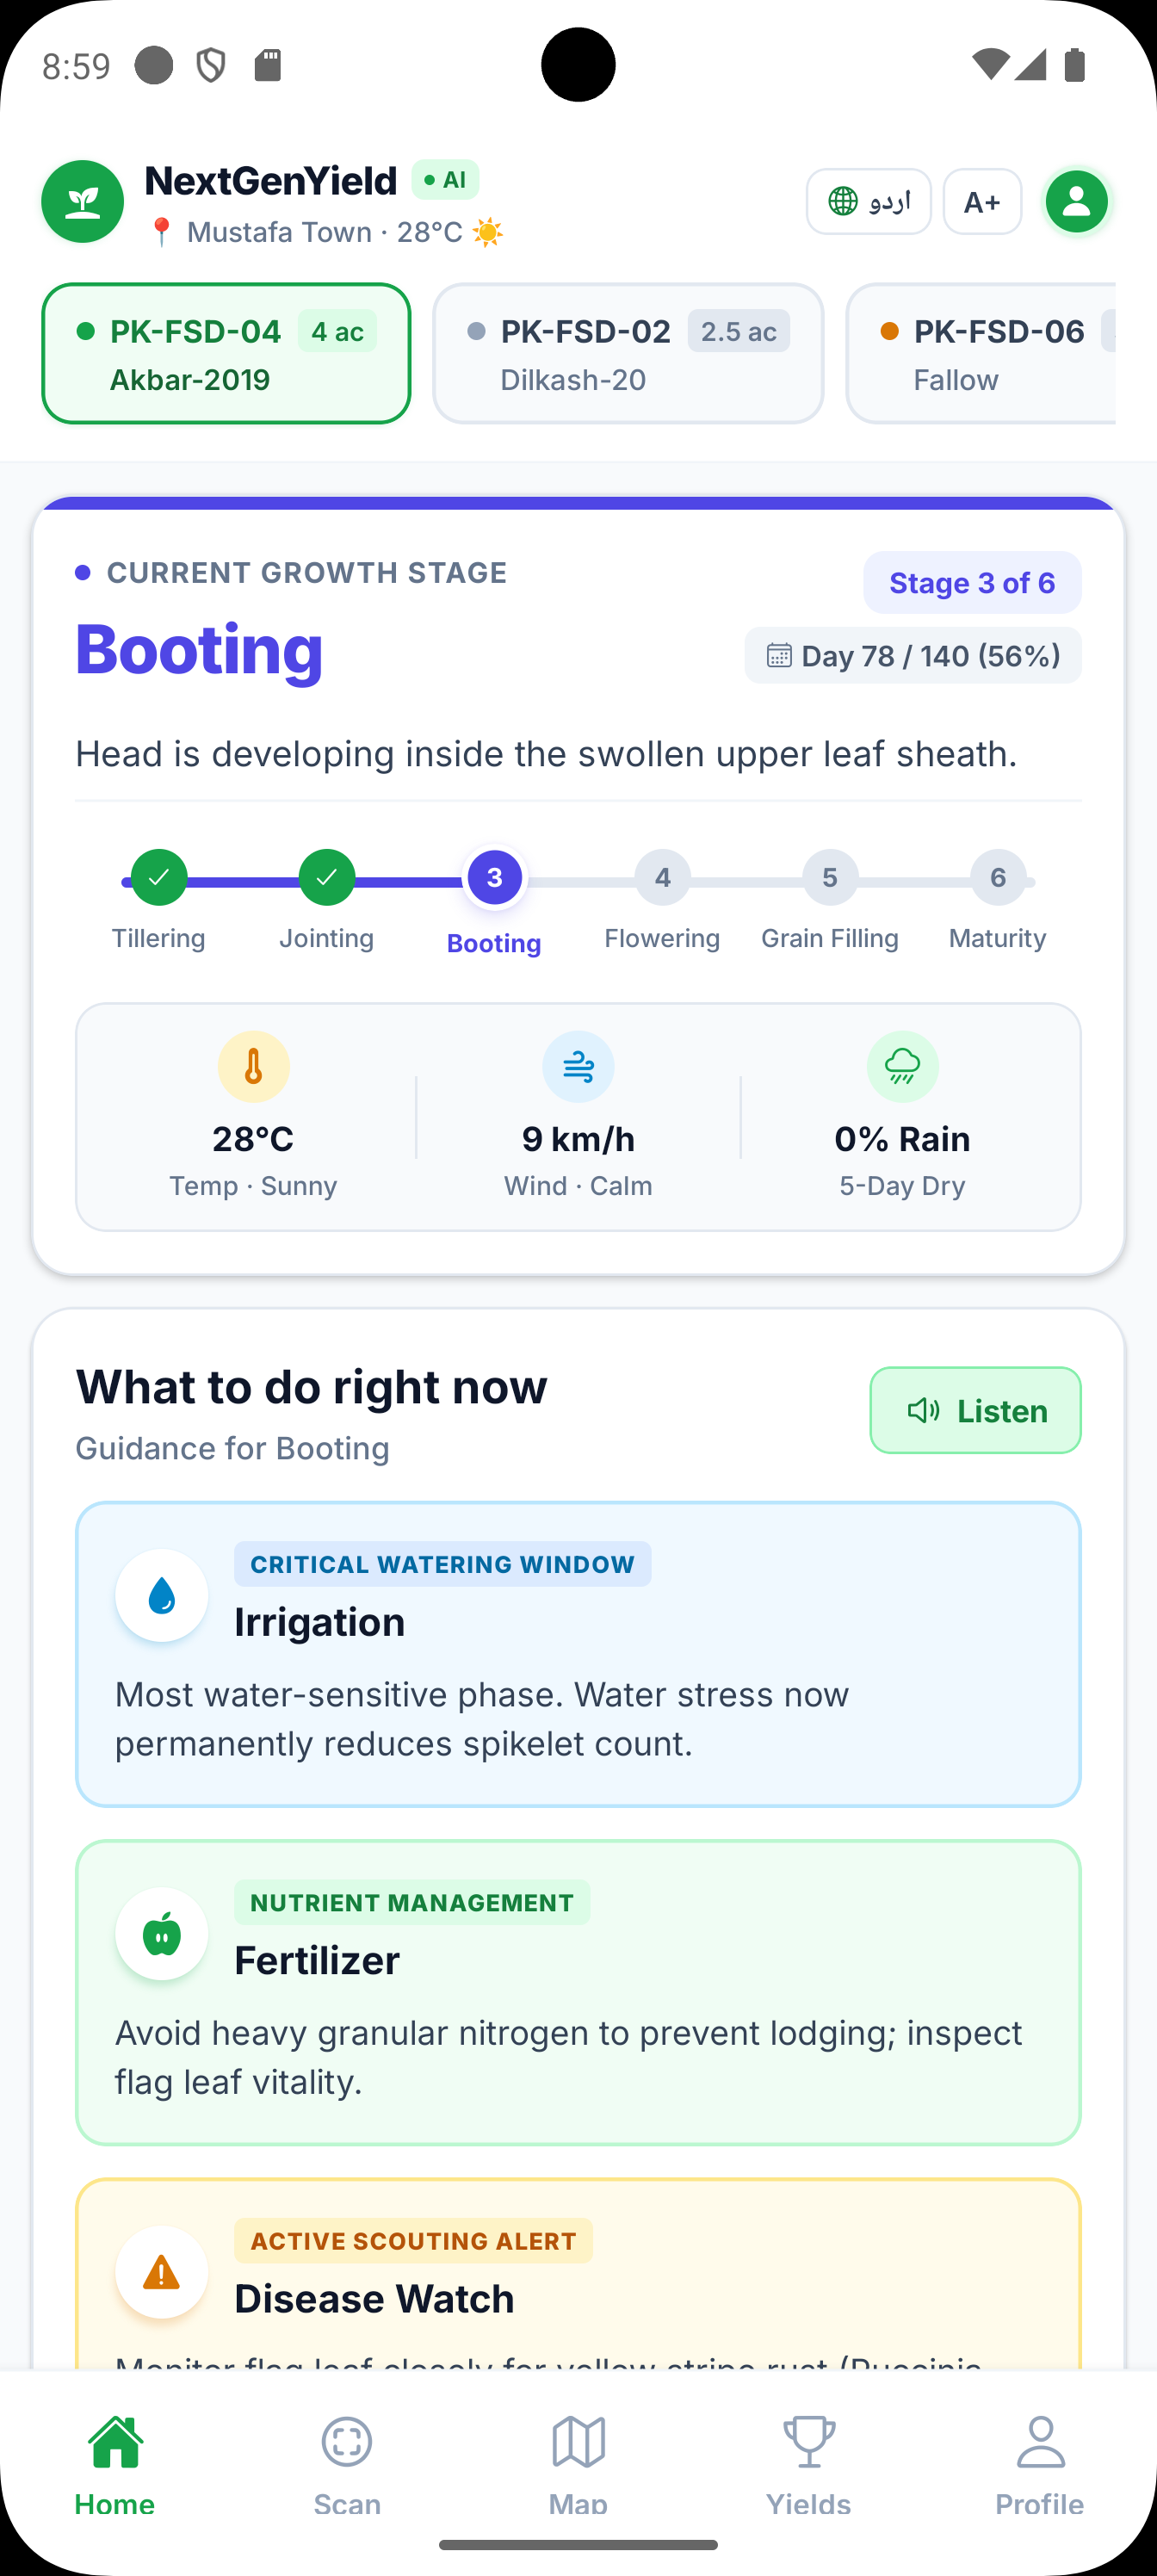
\includegraphics[draft=false, width=0.45\textwidth]{Figures/home_dashboard.png}
        \vspace{0.8em}
    \end{minipage}
}
\caption{Farmer Home Dashboard and Cycle Management View}
\label{fig:gui_dashboard}
\end{figure}

\begin{figure}[!htbp]
\centering
\fbox{
    \begin{minipage}{0.85\textwidth}
        \centering
        \vspace{0.8em}
        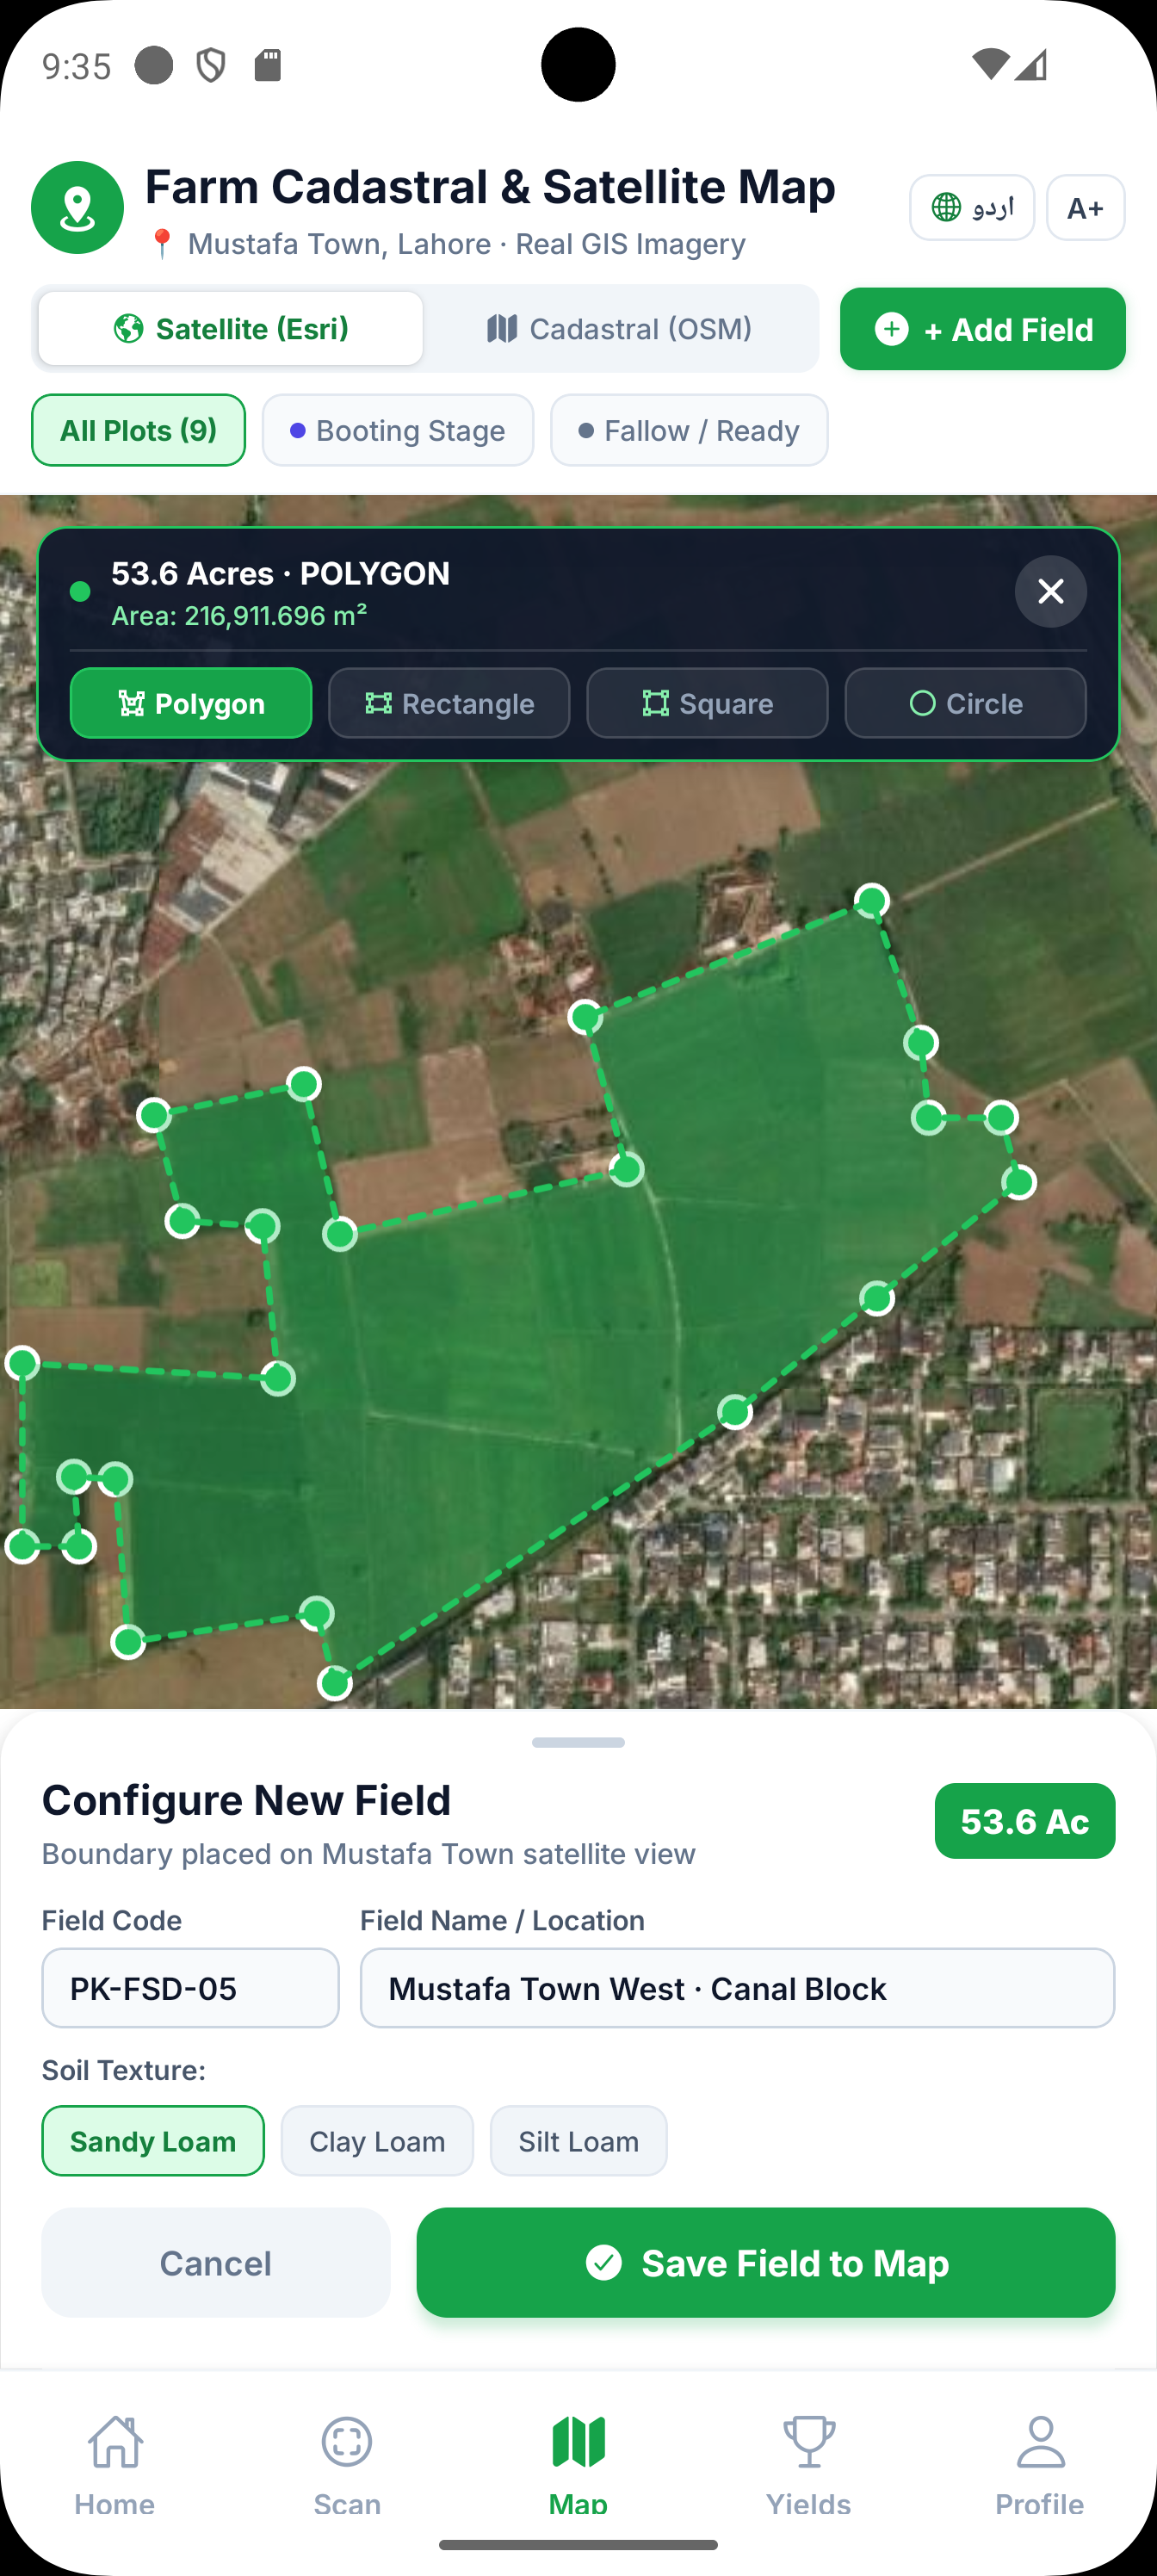
\includegraphics[draft=false, width=0.45\textwidth]{Figures/map_demarcation.png}
        \vspace{0.8em}
    \end{minipage}
}
\caption{Decoupled Interactive GeoJSON Map Demarcation Interface}
\label{fig:gui_dashboard}
\end{figure}

\begin{figure}[!htbp]
\centering
\fbox{
    \begin{minipage}{0.85\textwidth}
        \centering
        \vspace{0.8em}
        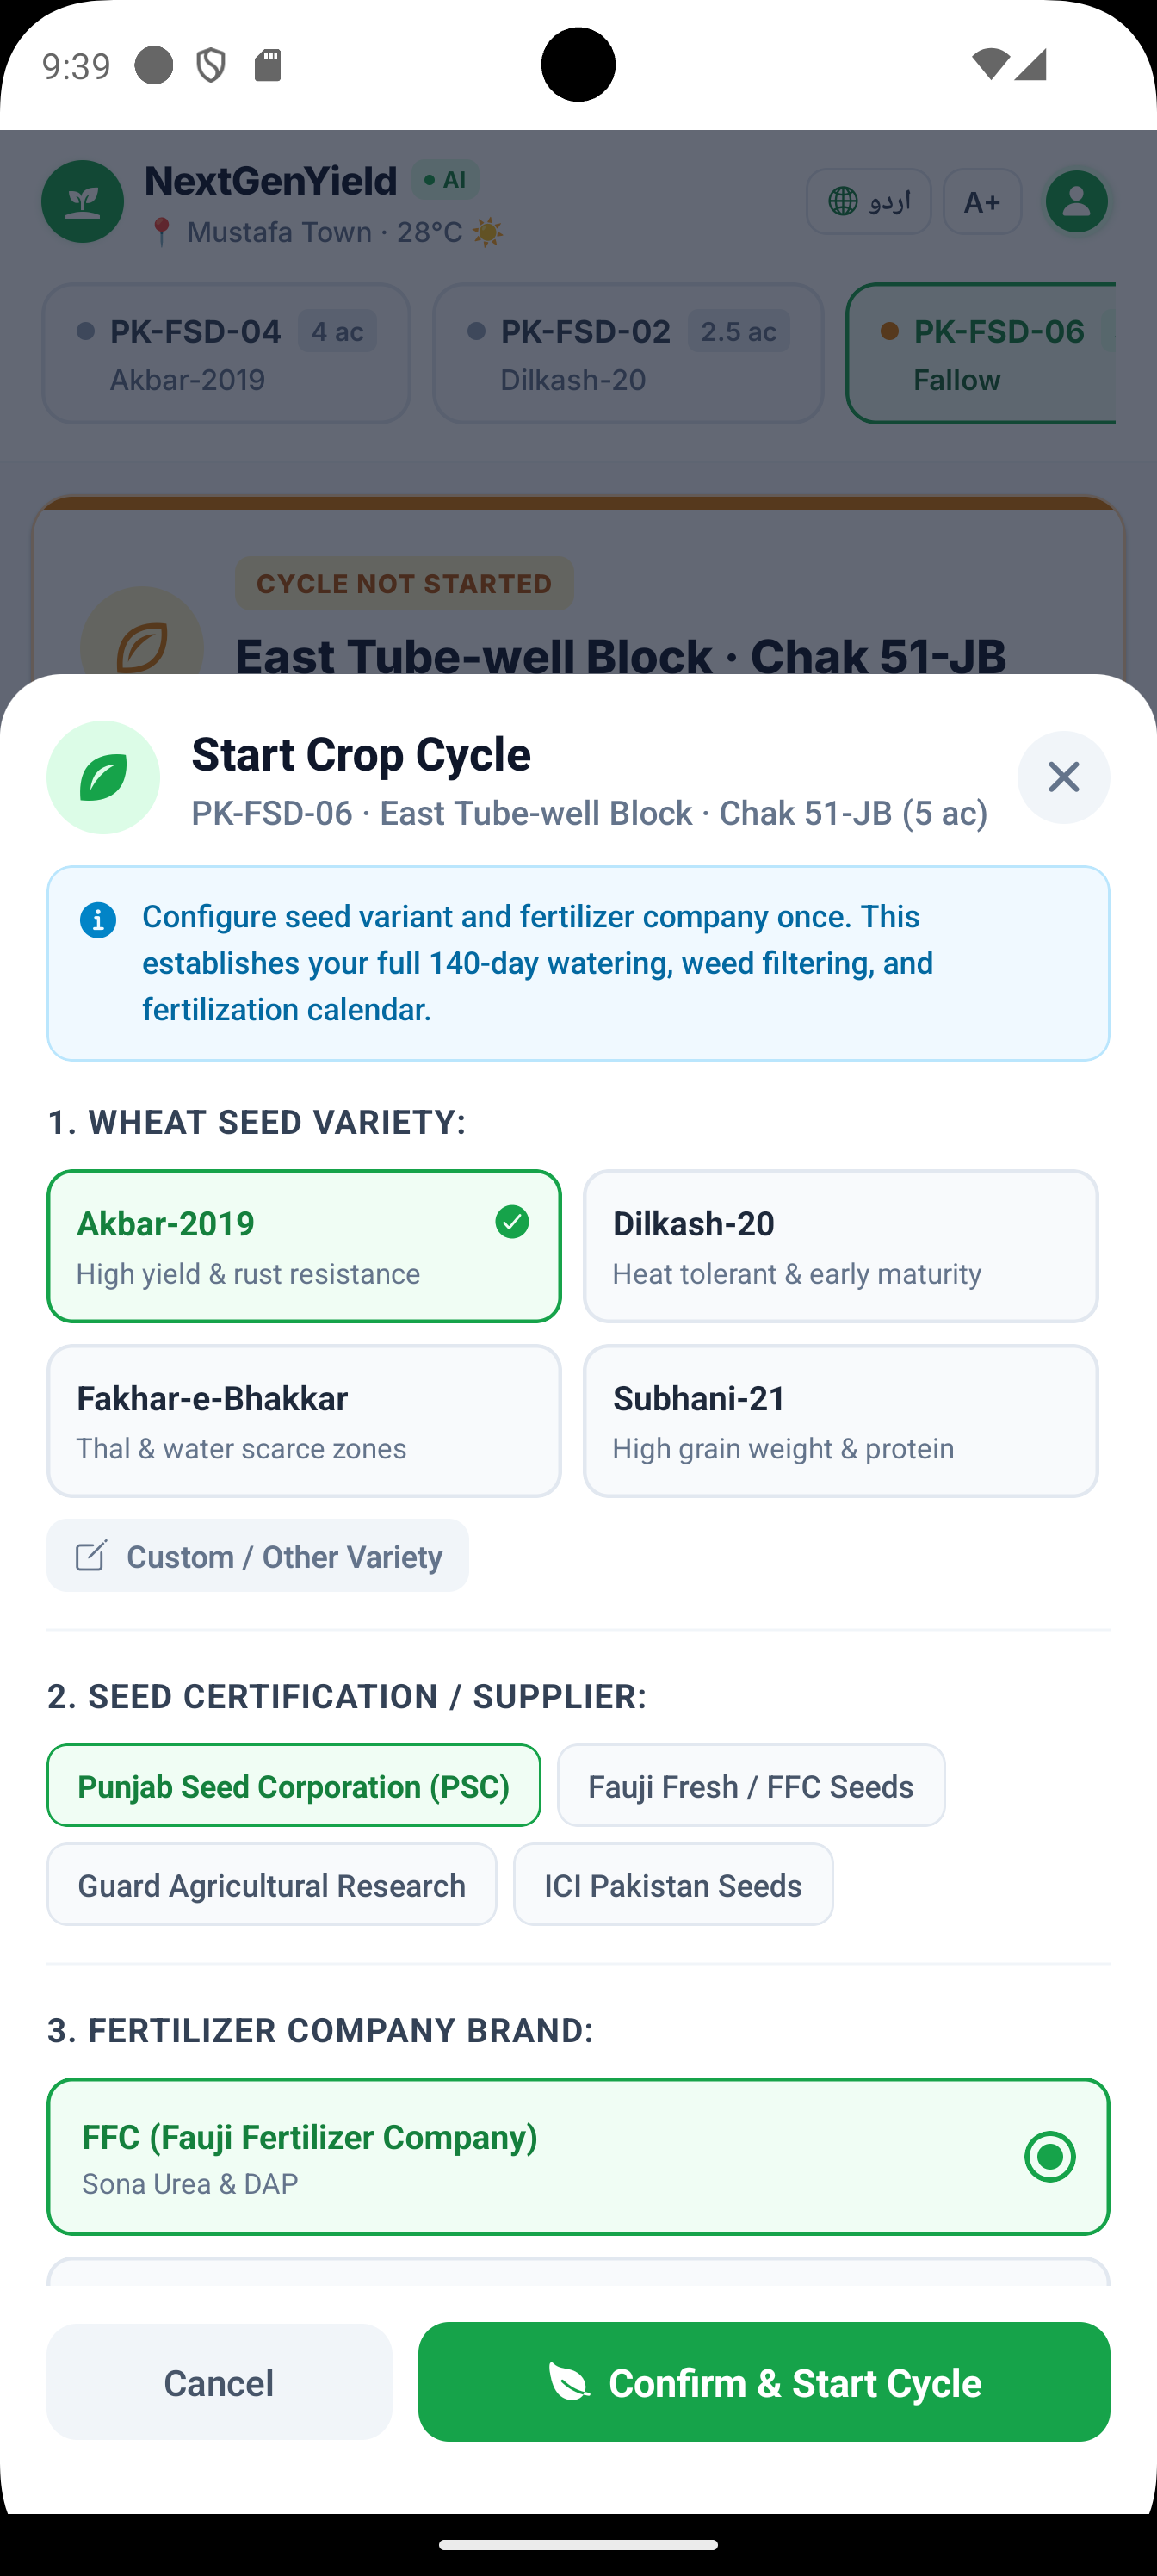
\includegraphics[draft=false, width=0.45\textwidth]{Figures/crop_cycle.png}
        \vspace{0.8em}
    \end{minipage}
}
\caption{Single-Entry Crop Cycle Initialization Modal}
\label{fig:gui_dashboard}
\end{figure}


\begin{figure}[!htbp]
\centering
\fbox{
    \begin{minipage}{0.85\textwidth}
        \centering
        \vspace{0.8em}
        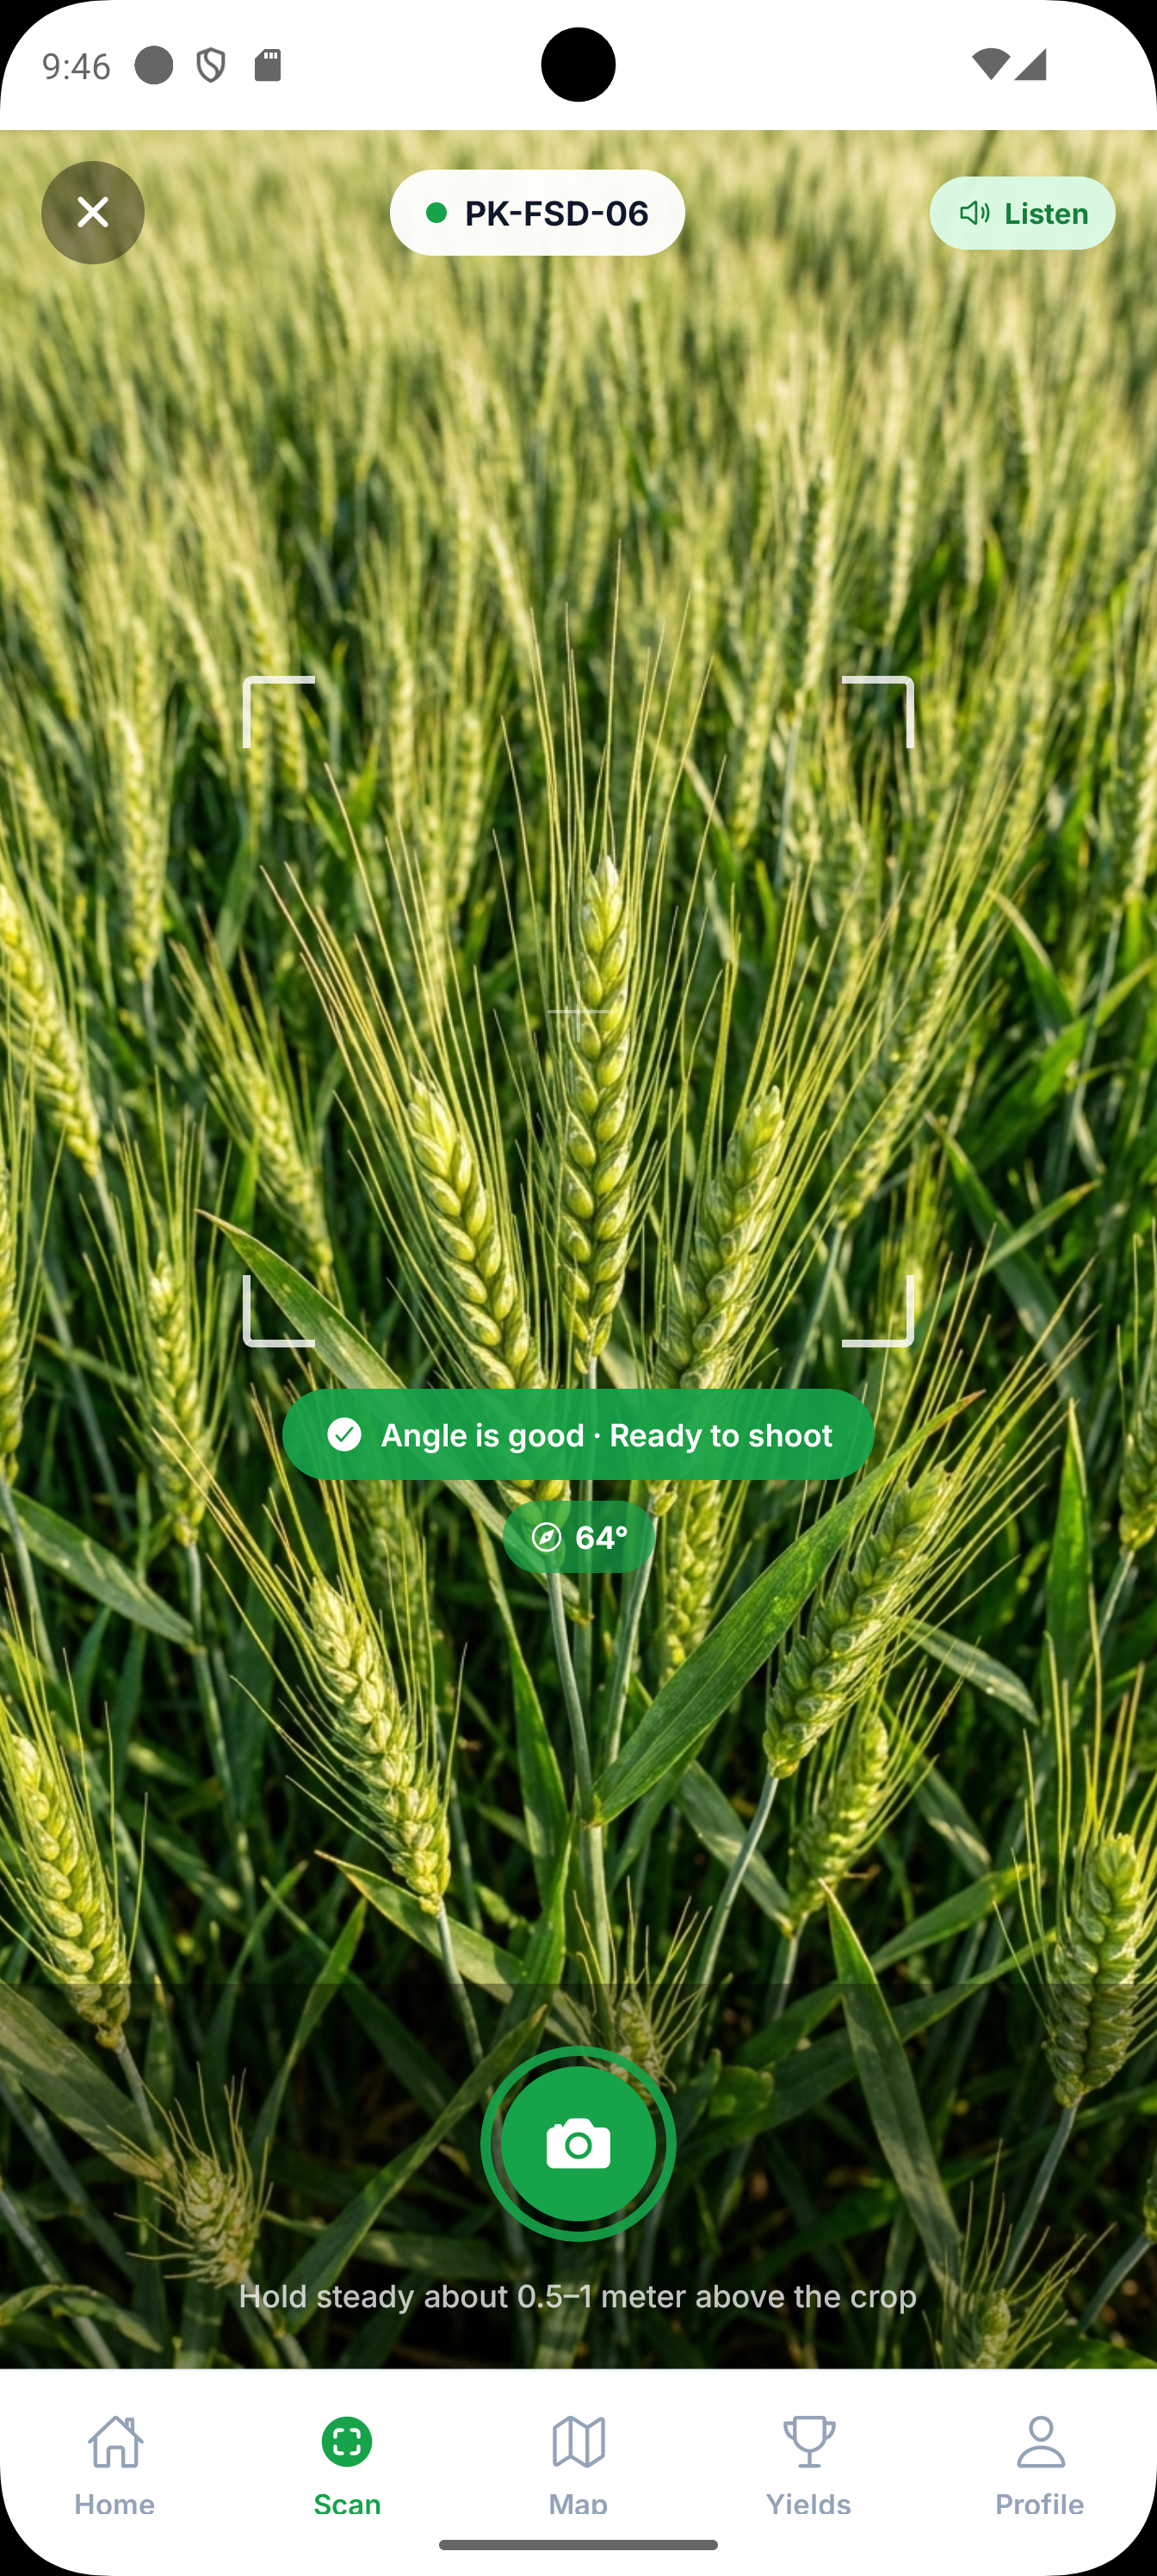
\includegraphics[draft=false, width=0.45\textwidth]{Figures/photography_guardrail.png}
        \vspace{0.8em}
    \end{minipage}
}
\caption{Modal guided Field Photography Guardrail}
\label{fig:gui_dashboard}
\end{figure}

\begin{figure}[!htbp]
\centering
\fbox{
    \begin{minipage}{0.85\textwidth}
        \centering
        \vspace{0.8em}
        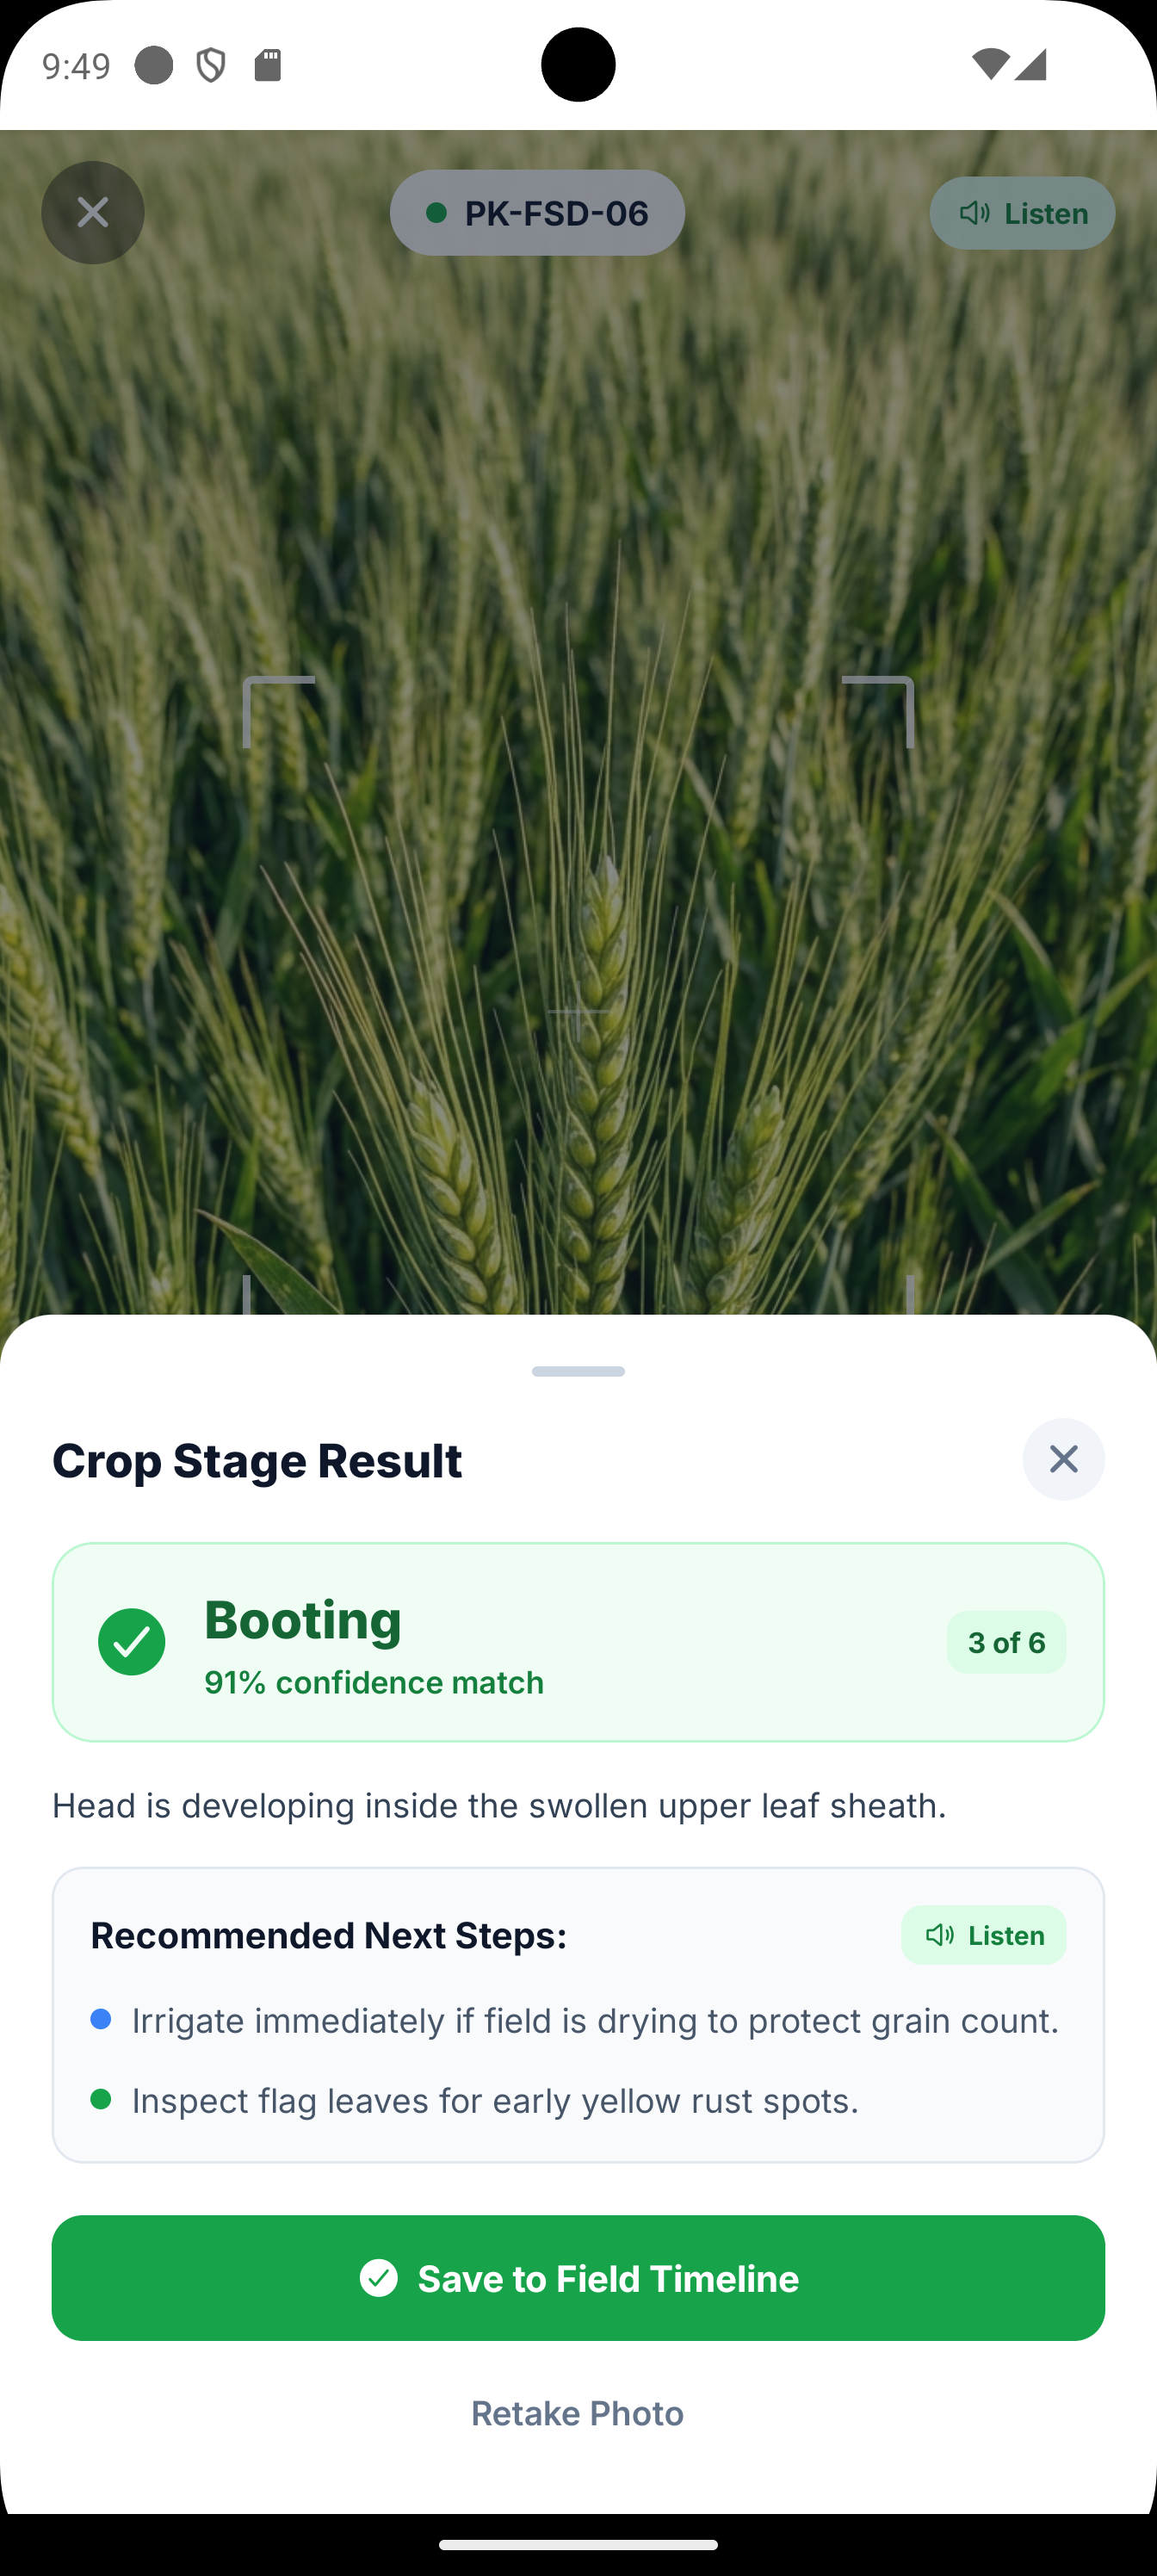
\includegraphics[draft=false, width=0.45\textwidth]{Figures/growth_stage.png}
        \vspace{0.8em}
    \end{minipage}
}
\caption{Phenological AI Classification and Agronomic Advisory Card}
\label{fig:gui_dashboard}
\end{figure}

\begin{figure}[!htbp]
\centering
\fbox{
    \begin{minipage}{0.85\textwidth}
        \centering
        \vspace{0.8em}
        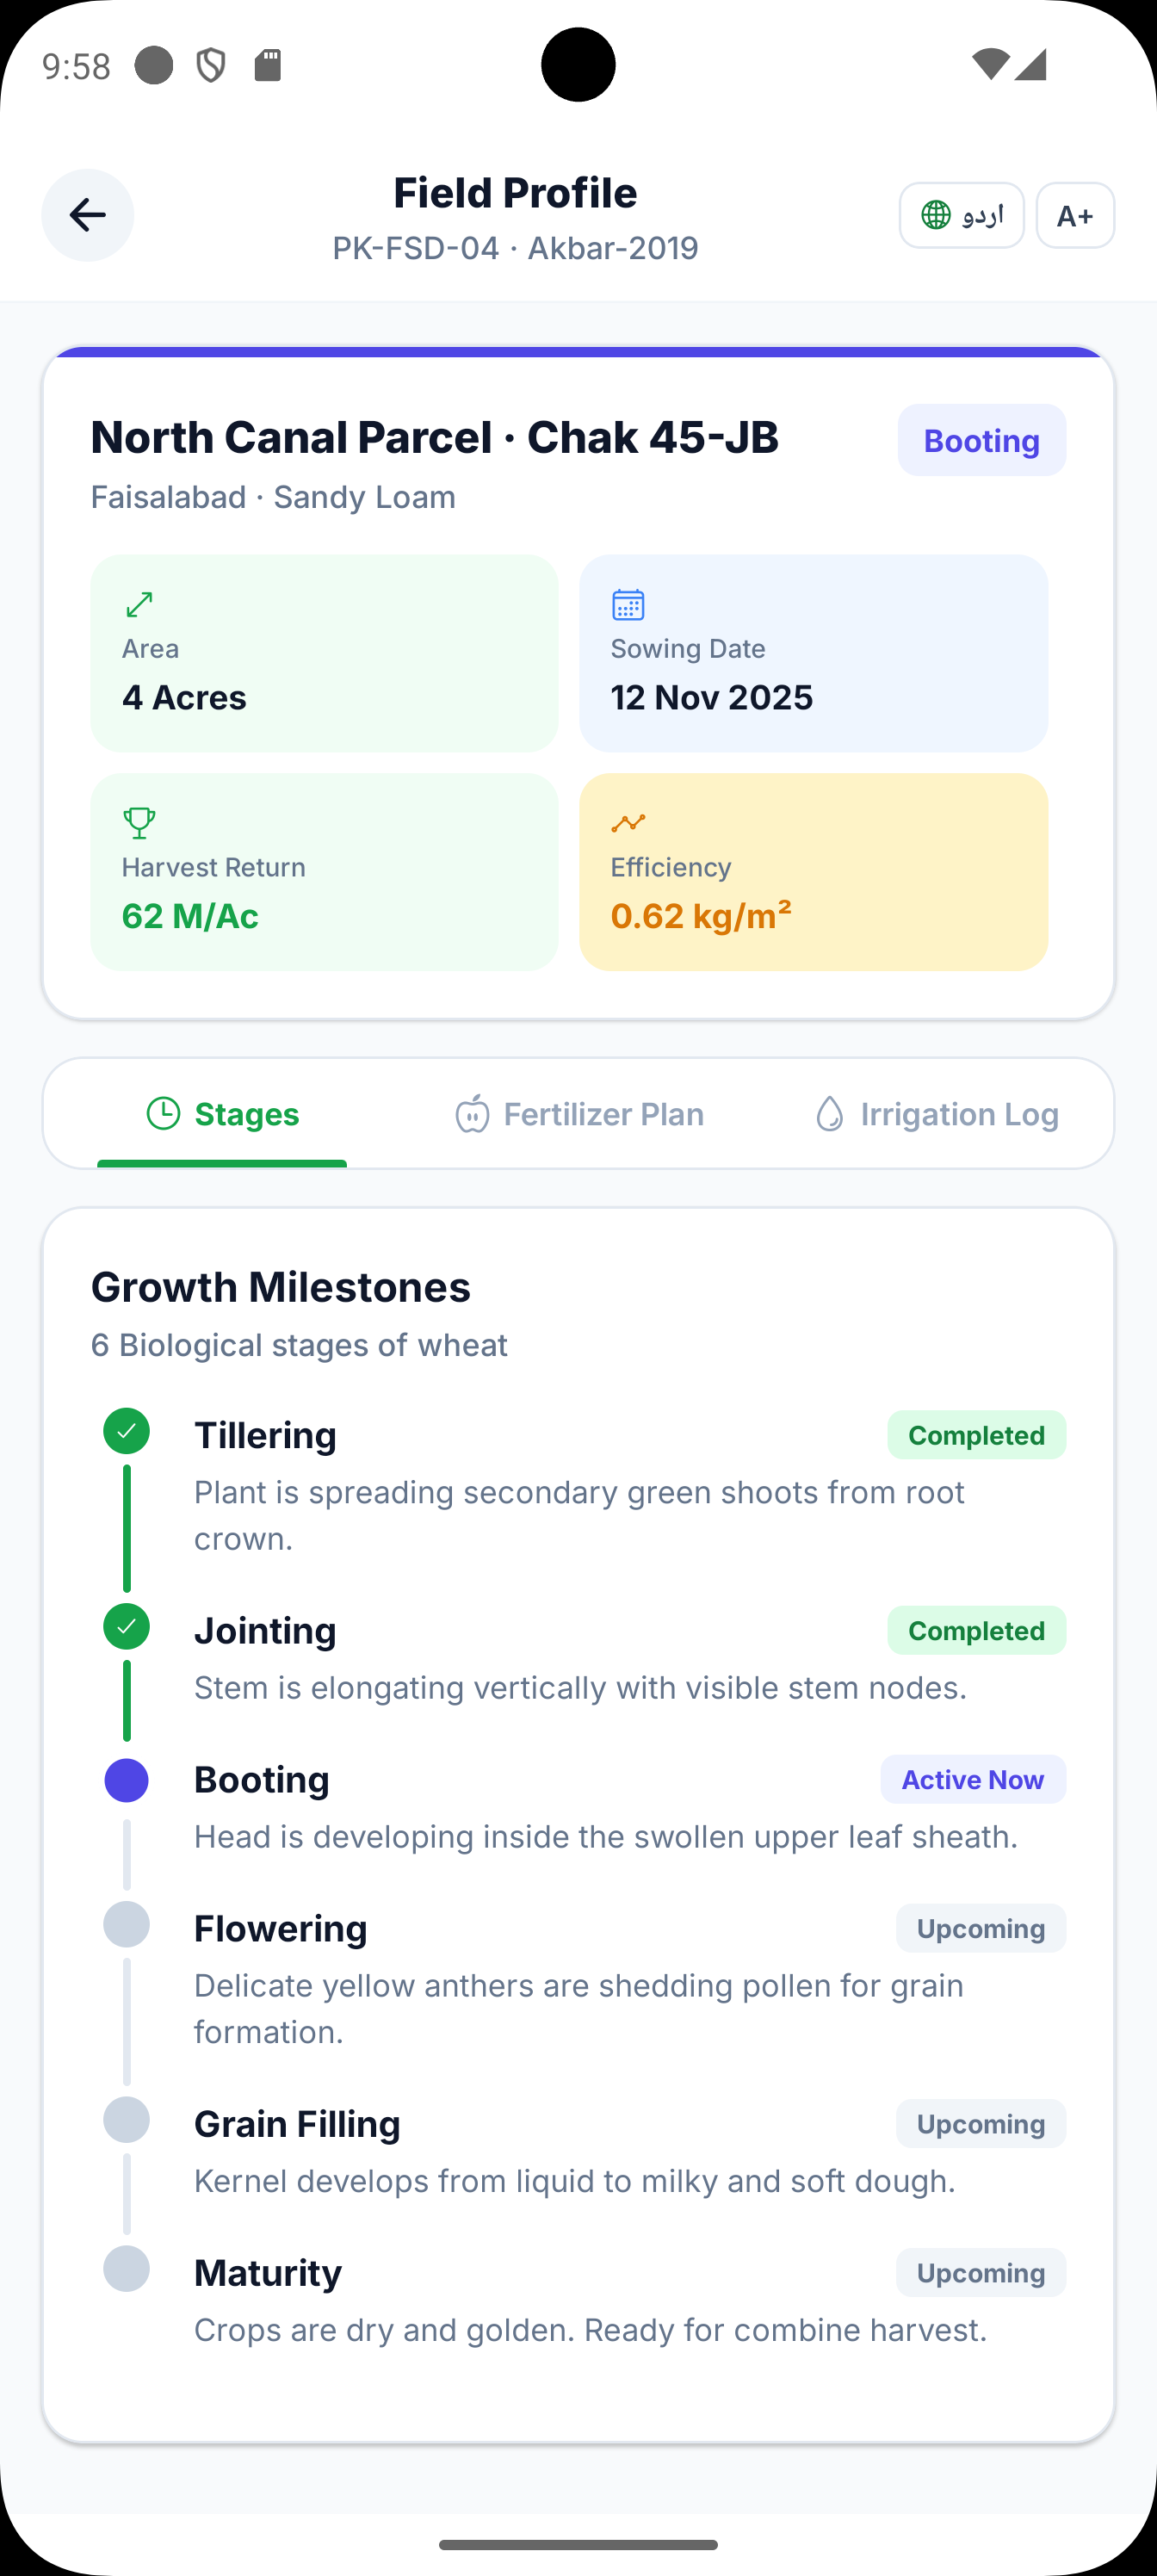
\includegraphics[draft=false, width=0.45\textwidth]{Figures/growth_timeline.png}
        \vspace{0.8em}
    \end{minipage}
}
\caption{Temporal Crop Growth Timeline Screen}
\label{fig:gui_dashboard}
\end{figure}

\begin{figure}[!htbp]
\centering
\fbox{
    \begin{minipage}{0.85\textwidth}
        \centering
        \vspace{0.8em}
        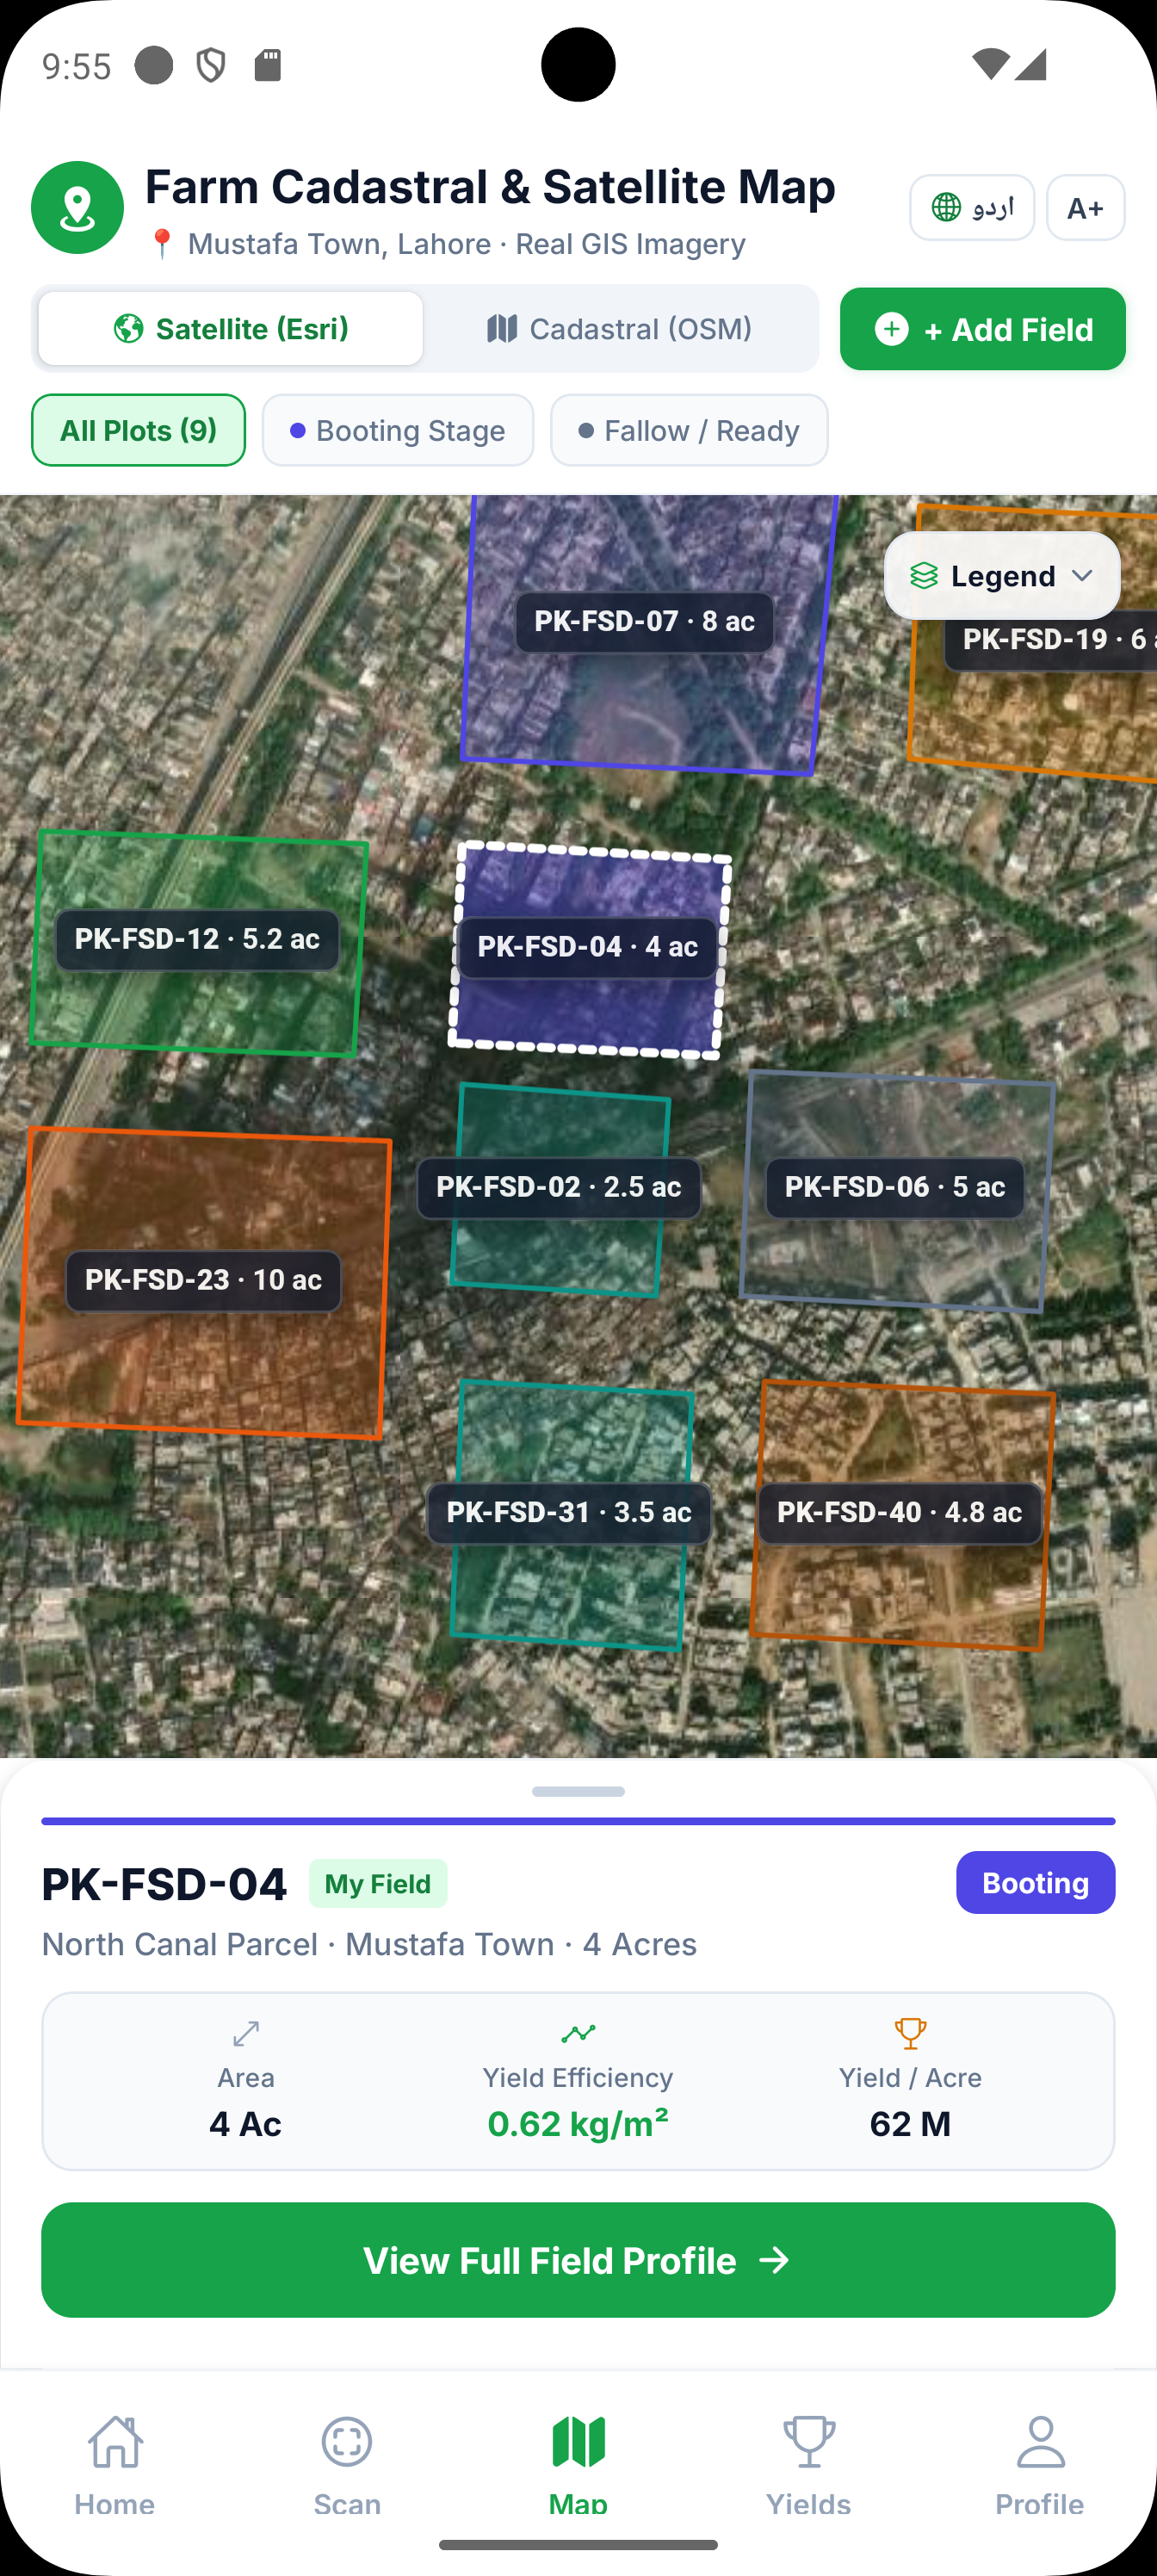
\includegraphics[draft=false, width=0.45\textwidth]{Figures/farm_network.png}
        \vspace{0.8em}
    \end{minipage}
}
\caption{Regional GIS Farm Network and Neighbor Plot Inspection}
\label{fig:gui_dashboard}
\end{figure}

\begin{figure}[!htbp]
\centering
\fbox{
    \begin{minipage}{0.85\textwidth}
        \centering
        \vspace{0.8em}
        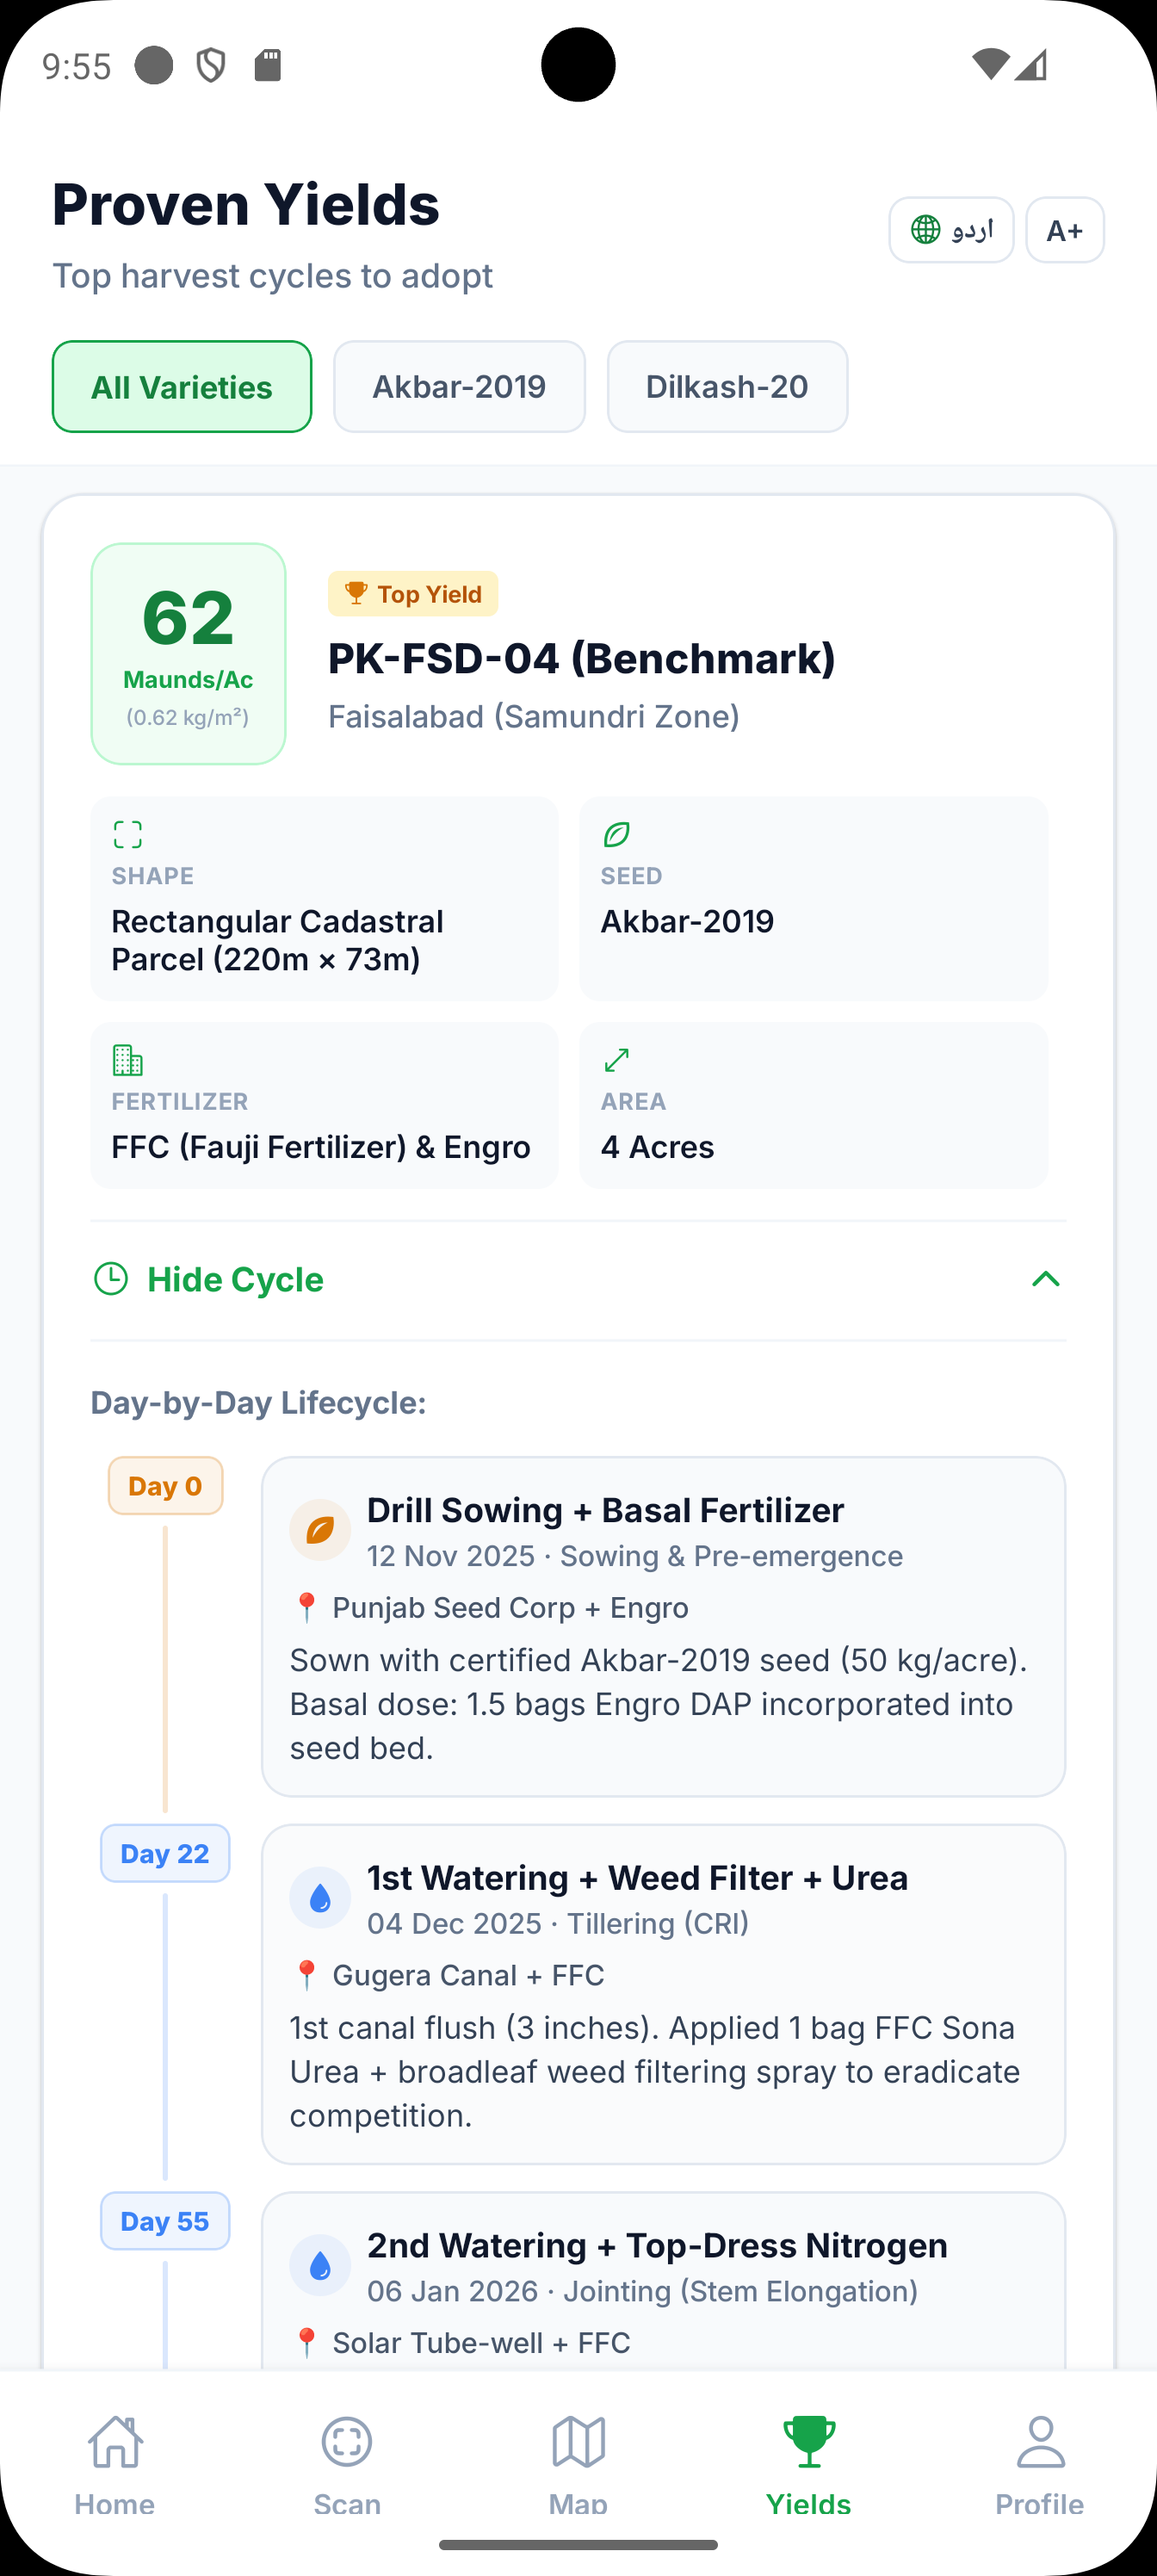
\includegraphics[draft=false, width=0.45\textwidth]{Figures/proven_yields.png}
        \vspace{0.8em}
    \end{minipage}
}
\caption{Proven Techniques Showcase and 140-Day Event Log}
\label{fig:gui_dashboard}
\end{figure}

\begin{figure}[!htbp]
\centering
\fbox{
    \begin{minipage}{0.85\textwidth}
        \centering
        \vspace{0.8em}
        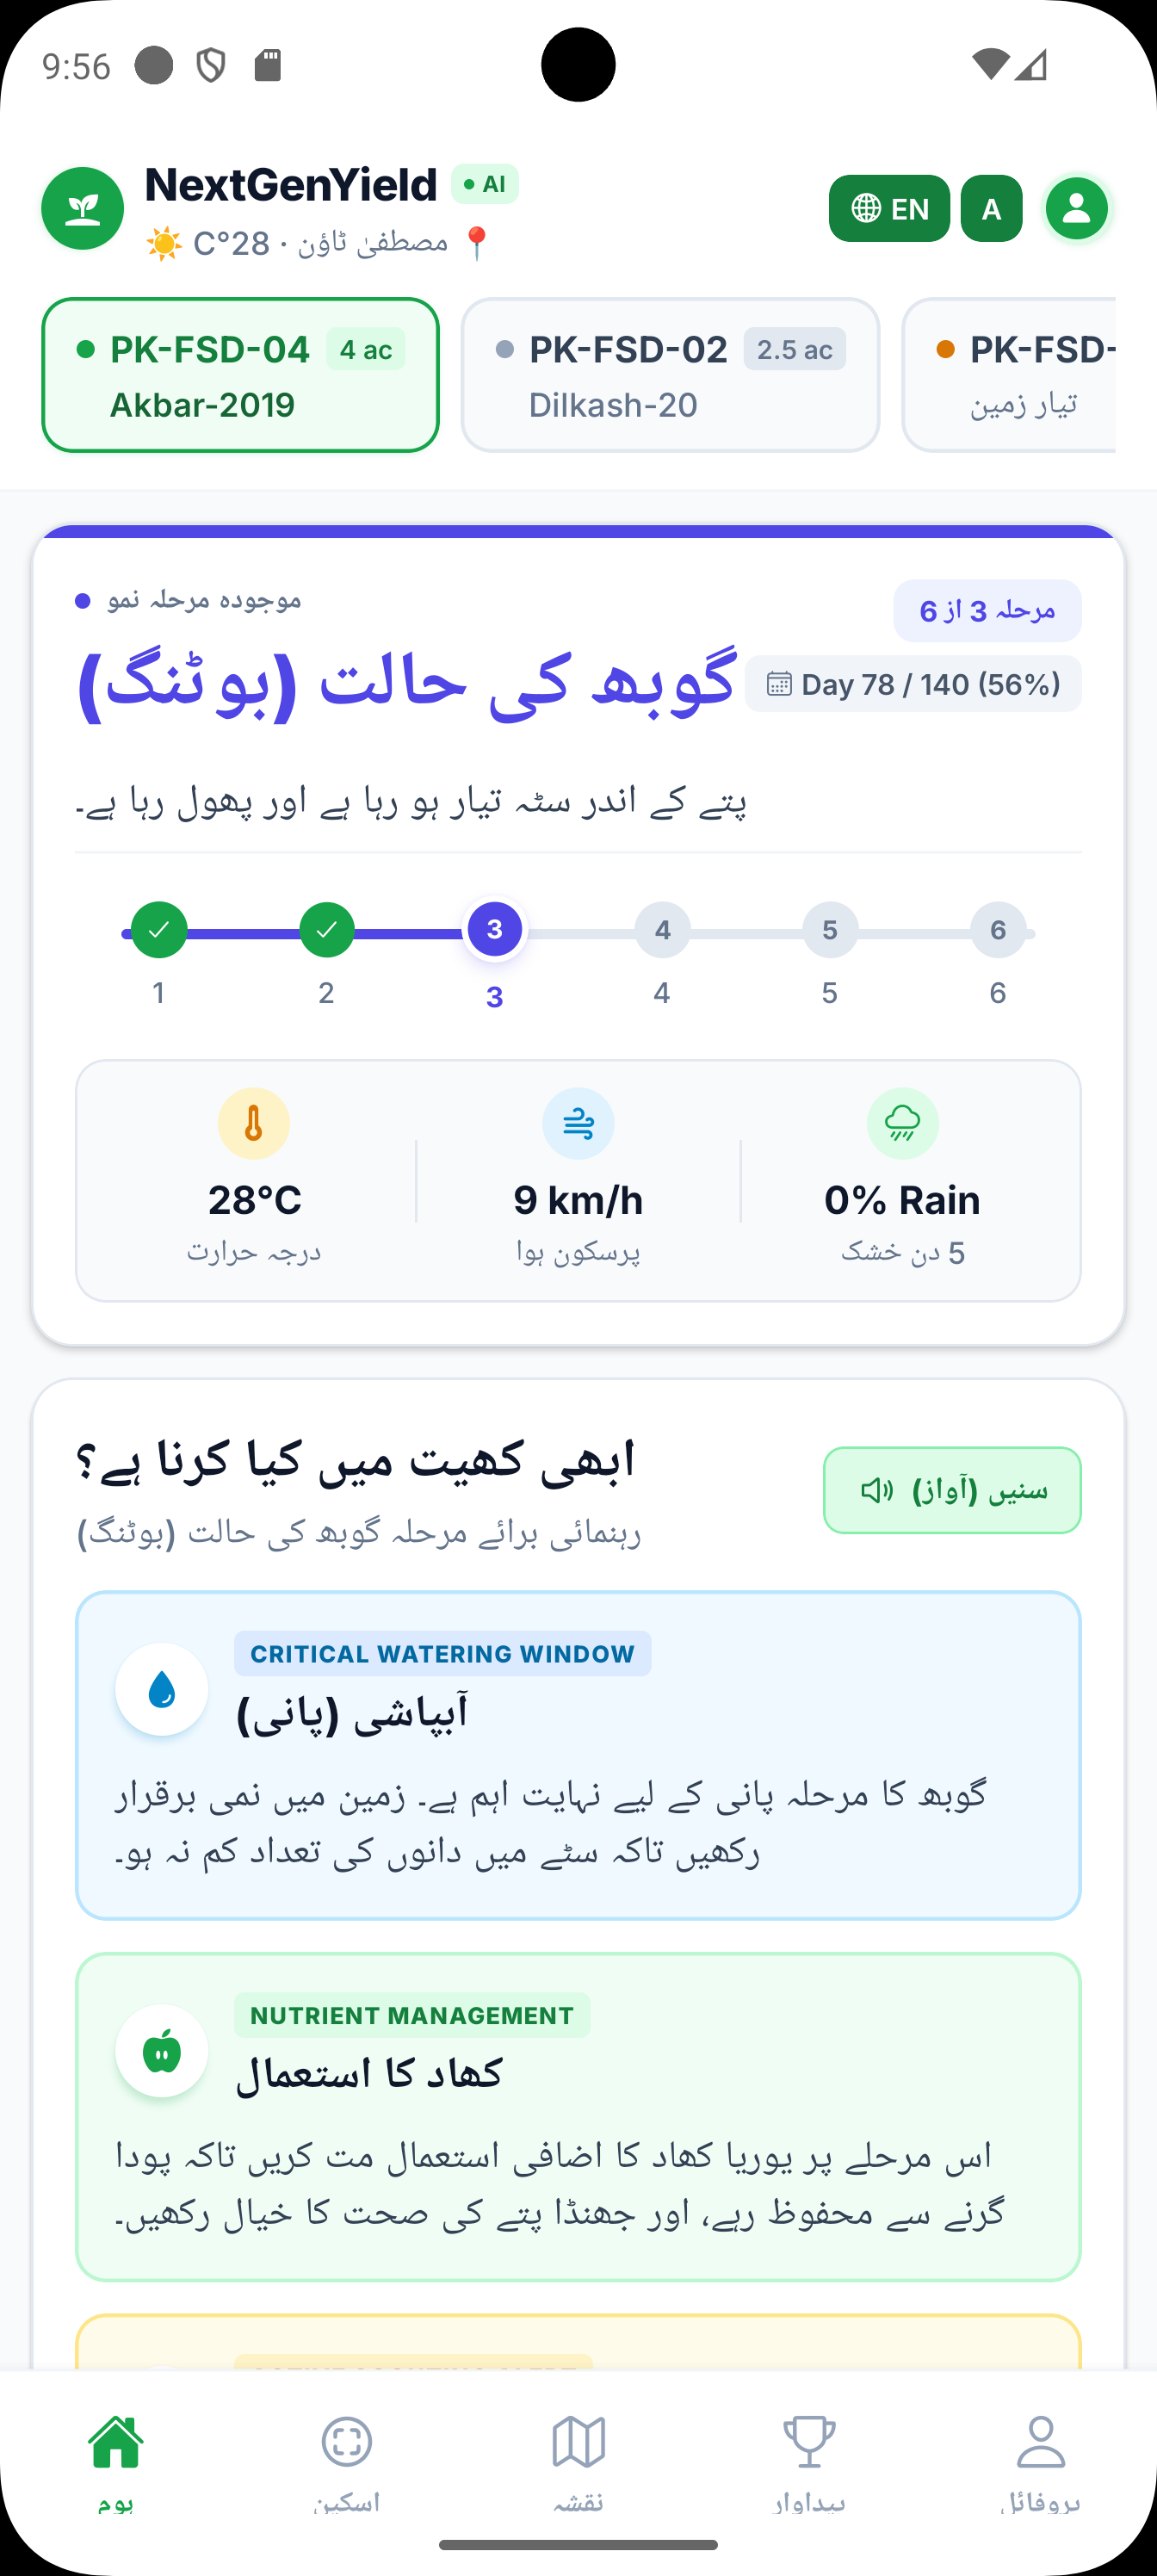
\includegraphics[draft=false, width=0.45\textwidth]{Figures/farmer_accessibility.png}
        \vspace{0.8em}
    \end{minipage}
}
\caption{Farmer Accessibility and Spoken Audio Narration Settings}
\label{fig:gui_dashboard}
\end{figure}



\clearpage
\section{Database Design}
The NextGenYield persistence layer is structured using a relational schema implemented in PostgreSQL with the PostGIS extension for geospatial polygon boundaries. The Entity-Relationship (ER) model and associated data dictionary tables are defined below.

\subsection{ER Diagram}
\begin{figure}[H]
\centering
\fbox{
    \parbox[c][6.5cm][c]{0.85\textwidth}{
        \centering
        \textbf{[Figure 4.10: Entity-Relationship Diagram of the NextGenYield Database]}\\[1em]
        \textit{\small (Placeholder: ER Diagram illustrating User, Field, CropCycle, FieldObservation, FertilizerSchedule, IrrigationSchedule, PeerShowcaseField, and AgronomicAdvisoryRule entities)}
    }
}
\caption{Entity-Relationship Diagram of the NextGenYield Database}
\label{fig:er_diagram}
\end{figure}

\subsection{Data Dictionary}
The relational database architecture is defined by the following eight entity specifications:

\begin{table}[H]
\footnotesize
\centering
\caption{User Table Data Dictionary}
\label{tab:user_table}
\begin{tabular}{|l|l|c|l|l|p{4.5cm}|}
\hline
\textbf{Attribute} & \textbf{Data Type} & \textbf{Null} & \textbf{Relation} & \textbf{Rel Type} & \textbf{Description} \\ \hline
UserID & Primary Key & No & - & - & Unique identifier for the user. \\ \hline
FullName & Varchar(60) & No & - & - & Full legal or preferred name of the user. \\ \hline
PhoneNumber & Varchar(15) & No & - & - & Primary contact number used for authentication. \\ \hline
PasswordHash & Varchar(255) & No & - & - & Bcrypt hashed security password/PIN. \\ \hline
Role & Varchar(20) & No & - & - & User role (`farmer', `landowner', `stakeholder'). \\ \hline
District & Varchar(50) & No & - & - & Home administrative district (e.g., Faisalabad). \\ \hline
LanguagePref & Varchar(5) & No & - & - & Language code (`ur' for Urdu, `en' for English). \\ \hline
CreatedAt & Timestamp & No & - & - & Record creation timestamp. \\ \hline
\end{tabular}
\end{table}

\begin{table}[H]
\footnotesize
\centering
\caption{Field Table Data Dictionary}
\label{tab:field_table}
\begin{tabular}{|l|l|c|l|l|p{4.5cm}|}
\hline
\textbf{Attribute} & \textbf{Data Type} & \textbf{Null} & \textbf{Relation} & \textbf{Rel Type} & \textbf{Description} \\ \hline
FieldID & Primary Key & No & - & - & Unique identifier for the land parcel. \\ \hline
UserID & Foreign Key & No & User & Many-to-One & User who owns or manages the field. \\ \hline
FieldName & Varchar(50) & No & - & - & Friendly display name (e.g., North Canal Plot). \\ \hline
ShapeType & Varchar(15) & No & - & - & Geometry type (`square', `rectangle', `polygon', `circle'). \\ \hline
AreaAcres & Decimal(6,2) & No & - & - & Computed land area in standard acres. \\ \hline
AreaSqm & Decimal(10,2) & No & - & - & Computed land area in square meters. \\ \hline
BoundaryGeoJSON & JSONB & No & - & - & RFC 7946 GeoJSON polygon coordinates. \\ \hline
CenterLatitude & Decimal(9,6) & No & - & - & Geographic centroid latitude coordinate. \\ \hline
CenterLongitude & Decimal(9,6) & No & - & - & Geographic centroid longitude coordinate. \\ \hline
CurrentCycleID & Foreign Key & Yes & CropCycle & One-to-One & Active crop cycle pointer (null if fallow). \\ \hline
CreatedAt & Timestamp & No & - & - & Record creation timestamp. \\ \hline
\end{tabular}
\end{table}

\begin{table}[H]
\footnotesize
\centering
\caption{CropCycle Table Data Dictionary}
\label{tab:cropcycle_table}
\begin{tabular}{|l|l|c|l|l|p{4.5cm}|}
\hline
\textbf{Attribute} & \textbf{Data Type} & \textbf{Null} & \textbf{Relation} & \textbf{Rel Type} & \textbf{Description} \\ \hline
CycleID & Primary Key & No & - & - & Unique identifier for the 140-day crop cycle. \\ \hline
FieldID & Foreign Key & No & Field & Many-to-One & Associated land parcel. \\ \hline
WheatVariety & Varchar(50) & No & - & - & Seed cultivar (Akbar-19, Dilkash-20, etc.). \\ \hline
SeedCompany & Varchar(60) & No & - & - & Certified seed provider or research agency. \\ \hline
FertilizerCompany & Varchar(60) & No & - & - & Partner manufacturer (FFC, Engro, Fatima). \\ \hline
SowingMethod & Varchar(30) & No & - & - & Planting method (Drill, Broadcast, Bed). \\ \hline
SowingDate & Date & No & - & - & Date seed was planted into moist soil. \\ \hline
TargetHarvestDate & Date & No & - & - & Projected 140-day maturity harvest date. \\ \hline
IsActive & Boolean & No & - & - & Flag indicating whether cycle is ongoing. \\ \hline
CreatedAt & Timestamp & No & - & - & Record creation timestamp. \\ \hline
\end{tabular}
\end{table}

\begin{table}[H]
\footnotesize
\centering
\caption{FieldObservation Table Data Dictionary}
\label{tab:observation_table}
\begin{tabular}{|l|l|c|l|l|p{4.5cm}|}
\hline
\textbf{Attribute} & \textbf{Data Type} & \textbf{Null} & \textbf{Relation} & \textbf{Rel Type} & \textbf{Description} \\ \hline
ObservationID & Primary Key & No & - & - & Unique identifier for visual scan record. \\ \hline
CycleID & Foreign Key & No & CropCycle & Many-to-One & Associated crop cycle. \\ \hline
ImageURI & Varchar(255) & No & - & - & Persistent file storage path for canopy photo. \\ \hline
StageIndex & Integer & No & - & - & Predicted stage index ($0$ to $5$). \\ \hline
StageName & Varchar(30) & No & - & - & Predicted stage label (e.g., Booting Stage). \\ \hline
Confidence & Decimal(5,2) & No & - & - & FoMo4Wheat classification confidence score (\%). \\ \hline
PitchAngleDeg & Decimal(4,1) & No & - & - & Measured camera pitch tilt angle ($45^\circ - 80^\circ$). \\ \hline
BlurScore & Decimal(6,2) & No & - & - & Laplacian edge variance sharpness metric. \\ \hline
DAS & Integer & No & - & - & Days After Sowing at time of capture. \\ \hline
CapturedAt & Timestamp & No & - & - & Exact timestamp of observation capture. \\ \hline
\end{tabular}
\end{table}

\begin{table}[H]
\footnotesize
\centering
\caption{FertilizerSchedule Table Data Dictionary}
\label{tab:fertilizer_table}
\begin{tabular}{|l|l|c|l|l|p{4.5cm}|}
\hline
\textbf{Attribute} & \textbf{Data Type} & \textbf{Null} & \textbf{Relation} & \textbf{Rel Type} & \textbf{Description} \\ \hline
FertilizerID & Primary Key & No & - & - & Unique identifier for fertilizer split entry. \\ \hline
CycleID & Foreign Key & No & CropCycle & Many-to-One & Associated crop cycle. \\ \hline
SplitNumber & Integer & No & - & - & Sequential application split ($1$, $2$, or $3$). \\ \hline
NutrientType & Varchar(40) & No & - & - & Type (e.g., Basal DAP, 1st Topdress Urea). \\ \hline
TargetDAS & Integer & No & - & - & Recommended Days After Sowing for application. \\ \hline
DosePerAcre & Varchar(50) & No & - & - & Recommended quantity (e.g., 1 Bag (50kg) / Acre). \\ \hline
IsApplied & Boolean & No & - & - & Flag indicating completed application. \\ \hline
AppliedAt & Timestamp & Yes & - & - & Timestamp of farmer confirmation. \\ \hline
\end{tabular}
\end{table}

\begin{table}[H]
\footnotesize
\centering
\caption{IrrigationSchedule Table Data Dictionary}
\label{tab:irrigation_table}
\begin{tabular}{|l|l|c|l|l|p{4.5cm}|}
\hline
\textbf{Attribute} & \textbf{Data Type} & \textbf{Null} & \textbf{Relation} & \textbf{Rel Type} & \textbf{Description} \\ \hline
IrrigationID & Primary Key & No & - & - & Unique identifier for irrigation event. \\ \hline
CycleID & Foreign Key & No & CropCycle & Many-to-One & Associated crop cycle. \\ \hline
EventName & Varchar(40) & No & - & - & Irrigation milestone (e.g., Rauni Pre-sowing, 1st CRI Irrigation). \\ \hline
WaterSource & Varchar(30) & No & - & - & Source (Canal Supply, Tube-well, Solar Pump). \\ \hline
TargetDAS & Integer & No & - & - & Target Days After Sowing (e.g., Day 22 for CRI). \\ \hline
IsCompleted & Boolean & No & - & - & Status indicating field watering completion. \\ \hline
\end{tabular}
\end{table}

\begin{table}[H]
\footnotesize
\centering
\caption{PeerShowcaseField Table Data Dictionary}
\label{tab:showcase_table}
\begin{tabular}{|l|l|c|l|l|p{4.5cm}|}
\hline
\textbf{Attribute} & \textbf{Data Type} & \textbf{Null} & \textbf{Relation} & \textbf{Rel Type} & \textbf{Description} \\ \hline
ShowcaseID & Primary Key & No & - & - & Unique identifier for verified benchmark plot. \\ \hline
FieldCode & Varchar(20) & No & - & - & Identifier (e.g., PK-FSD-04 Benchmark). \\ \hline
District & Varchar(50) & No & - & - & Agricultural tehsil/district (e.g., Samundri, Faisalabad). \\ \hline
WheatVariety & Varchar(50) & No & - & - & Wheat cultivar sown. \\ \hline
SeedCompany & Varchar(60) & No & - & - & Certified seed provider. \\ \hline
FertilizerCompany & Varchar(60) & No & - & - & Fertilizer manufacturer utilized. \\ \hline
AreaAcres & Decimal(6,2) & No & - & - & Total parcel acreage. \\ \hline
ShapeType & Varchar(15) & No & - & - & Geometry type (`rectangle', `square', `polygon', `circle'). \\ \hline
YieldMaundsPerAcre & Decimal(5,1) & No & - & - & Verified harvest yield (e.g., 62.0 Maunds/Acre). \\ \hline
YieldKgSqm & Decimal(5,2) & No & - & - & Normalized harvest yield efficiency ($\text{kg}/\text{m}^2$). \\ \hline
SowingDate & Date & No & - & - & Sowing date of the verified cycle. \\ \hline
HarvestDate & Date & No & - & - & Harvesting date of the verified cycle. \\ \hline
CycleEventLog & JSON & No & - & - & Full chronological 140-day log of watering, weed filtering, and fertilizer splits. \\ \hline
\end{tabular}
\end{table}

\begin{table}[H]
\footnotesize
\centering
\caption{AgronomicAdvisoryRule Table Data Dictionary}
\label{tab:advisory_table}
\begin{tabular}{|l|l|c|l|l|p{4.5cm}|}
\hline
\textbf{Attribute} & \textbf{Data Type} & \textbf{Null} & \textbf{Relation} & \textbf{Rel Type} & \textbf{Description} \\ \hline
RuleID & Primary Key & No & - & - & Unique identifier for deterministic rule. \\ \hline
StageIndex & Integer & No & - & - & Biological wheat growth stage index ($0$ to $5$). \\ \hline
StageName & Varchar(30) & No & - & - & Growth stage identifier (Tillering, Booting, etc.). \\ \hline
SummaryTextEn & Text & No & - & - & English agronomic stage summary. \\ \hline
SummaryTextUr & Text & No & - & - & Urdu translated stage summary. \\ \hline
IrrigationAdviceEn & Text & No & - & - & English stage-specific watering directive. \\ \hline
IrrigationAdviceUr & Text & No & - & - & Urdu stage-specific watering directive. \\ \hline
NutrientAdviceEn & Text & No & - & - & English fertilizer timing guidance. \\ \hline
NutrientAdviceUr & Text & No & - & - & Urdu fertilizer timing guidance. \\ \hline
RiskAlerts & JSON & No & - & - & Active disease/weather hazard warnings array. \\ \hline
AudioScriptUr & Text & No & - & - & Phonetic Urdu audio synthesis script. \\ \hline
\end{tabular}
\end{table}

\clearpage
\section{Risk Analysis}
Risk assessment and management are foundational to ensuring NextGenYield's agronomic validity, operational resilience, and sustained adoption among smallholder farming communities. The principal risk dimensions and mitigation protocols are outlined below.

\subsection{Technical and Environmental Vision Risks}
\begin{itemize}
    \item \textbf{Risk Description:} Outdoor agricultural photography is subject to severe environmental degradation, including wind-induced plant motion blur, intense direct solar glare ($> 60,000\text{ lux}$), shadow occlusions, and off-target horizontal camera angles pointing at weed foliage or lateral stems.
    \item \textbf{Mitigation Strategy:} NextGenYield implements on-device sensor fusion. Real-time accelerometer and gyroscope listeners enforce a strict downward pitch angle reticle ($45^\circ - 80^\circ$) before camera activation, and an edge Laplacian variance filter halts capture if motion blur exceeds thresholds ($< 90$). This guarantees that only crisp canopy imagery enters the vision pipeline.
\end{itemize}

\subsection{Agronomic Safety and Misinformation Risks}
\begin{itemize}
    \item \textbf{Risk Description:} Automated agricultural advisory systems that deploy ungrounded Large Language Models (LLMs) are prone to hallucinations, generating fabricated chemical formulations, premature irrigation advice during high winds, or excessive nitrogen dosages that trigger vegetative lodging and ground-water leaching.
    \item \textbf{Mitigation Strategy:} NextGenYield eliminates probabilistic generative text models from the advisory pathway. Growth stage classifications are linked directly to deterministic, verified agronomic rule tables reviewed by certified agronomic research institutions.
\end{itemize}

\subsection{User Adoption and Human Factors Risks}
\begin{itemize}
    \item \textbf{Risk Description:} Smallholder farmers in the Punjab agricultural belt frequently possess limited English literacy and smartphone experience. An overly complex, text-heavy interface risks complete abandonment or user error.
    \item \textbf{Mitigation Strategy:} The mobile user experience is designed with high visual contrast, intuitive icon metaphors, complete Urdu localization, and an integrated spoken Urdu audio synthesis player that narrates recommendations aloud at a single tap.
\end{itemize}

\subsection{Rural Telecommunications and Connectivity Risks}
\begin{itemize}
    \item \textbf{Risk Description:} Remote agricultural parcels frequently suffer from weak, intermittent $2\text{G}/3\text{G}$ cellular signals, causing network timeouts and data transmission failures during field operations.
    \item \textbf{Mitigation Strategy:} The application incorporates offline-first local caching. Field boundaries, stage advisory guidelines, and photographic records are stored on-device in persistent local storage. Captured observations are queued and automatically synchronized once cellular reception is re-established.
\end{itemize}

\subsection{Geospatial Demarcation and Land Discrepancy Risks}
\begin{itemize}
    \item \textbf{Risk Description:} Smallholder farms in Pakistan are subdivided into irregular, non-standard cadastral parcels (killas and acres) often bisected by irrigation canals, rendering rigid rectangular bounding tools ineffective.
    \item \textbf{Mitigation Strategy:} NextGenYield provides flexible multi-vertex polygon and centre-pivot circular boundary tools in addition to square and rectangular boxes, enabling farmers to accurately outline irregular parcels along irrigation watercourses and roads.
\end{itemize}

\clearpage
\section{Conclusion}
Chapter 4 has articulated the complete Software Requirement Specifications for NextGenYield. Beginning with a detailed feature breakdown and functional requirements for farmers, agricultural professionals, and backend systems, the chapter delineated non-functional performance and accessibility mandates. The nine formal use cases capture the end-to-end user journey---from GeoJSON boundary demarcation on satellite maps and single-entry cycle initialization to sensor-guided canopy photography, deterministic advisory generation, and peer benchmark replication. The graphical user interface architecture and relational database schema provide concrete implementation structures, while the risk analysis outlines rigorous mitigation strategies against vision degradation, agronomic hallucinations, and rural connectivity challenges. Together, these specifications lay an unyielding engineering foundation for precision wheat monitoring and decision support.

\chapter{Proposed Approach and Methodology}
The proposed approach could be a Framework, Heuristic, Algorithm, Protocol, or Mathematical-model.
For each chapter, provide a paragraph of introduction and in the end a paragraph of conclusions. Not the programming code but the algorithmic and procedural details especially related to the hidden/ backend algorithms that are not covered in the design.\\
\textcolor{red}{NOTE: This chapter is optional for Development projects but compulsory for Research projects.} 
\chapter{High-Level and Low-Level Design}
Provide the high- and low-level design of your system in this chapter. Select the design that is appropriate for your project.\\
\textcolor{red}{NOTE: This Chapter is compulsory for both R\&D projects and Development projects.}
\section{System Overview}
Provide a general description of the software system, including its functionality and matters related to the overall system and its design (perhaps including a discussion of the basic design approach or organization). Feel free to split this discussion up into subsections (and sub-subsections, etc. ...).
\section{Design Considerations}
This section describes many issues that need to be addressed or resolved before attempting to devise a complete design solution.
\subsection{Assumptions and Dependencies}
Describe any assumptions or dependencies regarding the software and its use. These may concern such issues as:
\begin{itemize}
\item Related software or hardware 
  \item Operating systems 
  \item End-user characteristics 
  \item Possible and/or probable changes in functionality
\end{itemize}
Do not just add random generic statements, be clear and concise about what you are writing.
\subsection{General Constraints}
Describe any global limitations or constraints that have a significant impact on the design of the system's software (and describe the associated impact). Such constraints may be imposed by any of the following (the list is not exhaustive):
\begin{itemize}
\item Hardware or software environment 
\item End-user environment 
\item Availability or volatility of resources 
\item Standards compliance 
\item Interoperability requirements 
\item Interface/protocol requirements 
\item Data repository and distribution requirements 
\item Security requirements (or other such regulations) 
\item Memory and other capacity limitations 
\item Performance requirements 
\item Network communications 
\item Verification and validation requirements (testing) 
\item Other means of addressing quality goals 
\item Other requirements described in the requirements specification 
\end{itemize}

\subsection{Goals and Guidelines}
Describe any goals, guidelines, principles, or priorities which dominate or embody the design of the system's software. Such goals might be:
\begin{itemize}
\item The KISS principle ("Keep it simple stupid!") 
\item Emphasis on speed versus memory use 
\item Working, looking, or "feeling" like an existing product
\end{itemize}
For each such goal or guideline, unless it is implicitly obvious, describe the reason for its desirability. Feel free to state and describe each goal in its own sub subsection if you wish.
\subsection{ Development Methods}
Briefly describe the method or approach used for this software design. If one or more formal/published methods were adopted or adapted, then include a reference to a more detailed description of these methods. If several methods were seriously considered, then each such method should be mentioned, along with a brief explanation of why all or part of it was used or not used.
\section{System Architecture}
This section should describe both the internal architecture of the modules, as well as the external architecture of the system with other systems, if any. Diagrammatic architecture is compulsory.\\
This section should provide a high-level overview of how the functionality and responsibilities of the system were partitioned and then assigned to subsystems or components. Do not go into too much detail about the individual components themselves (there is a subsequent section for detailed component descriptions). The main purpose here is to gain a general understanding of how and why the system was decomposed, and how the individual parts work together to provide the desired functionality.\\
At the top-most level, describe the major responsibilities that the software must undertake and the various roles that the system (or portions of the system) must play. Describe how the system was broken down into its components/subsystems (identifying each top-level component/subsystem and the roles/responsibilities assigned to it). Describe how the higher-level components collaborate with each other in order to achieve the required results. Don't forget to provide some sort of rationale for choosing this particular decomposition of the system (perhaps discussing other proposed decompositions and why they were rejected). Feel free to make use of design patterns, either in describing parts of the architecture (in pattern format), or for referring to elements of the architecture that employ them.\\
If there are any diagrams, models, flowcharts, documented scenarios or use-cases of the system behavior and/or structure, they may be included here (unless you feel they are complex enough to merit being placed in the Detailed System Design section). Diagrams that describe a particular component or sub-system should be included within the particular subsection that describes that component or subsystem.\\
\textcolor{red}{Note: This section (and its subsections) really applies only to newly developed (or yet-to-be developed) portions of the system.} If there are parts of the system that already existed before this development effort began, then you only need to describe the pre-existing parts that the new parts of the system depend upon, and only in enough detail sufficient to describe the relationships and interactions between the old parts and the new parts. Pre-existing parts that are modified or enhanced need to be described only to the extent that is necessary for the reader to gain a sufficient understanding of the nature of the changes that were made.
\subsection{Subsystem Architecture}
If a particular component is one which merits a more detailed discussion than what was presented in the System Architecture section, provide that more detailed discussion in a subsection of the System Architecture section (or it may even be more appropriate to describe the component in its own design document). If necessary, describe how the component was further divided into subcomponents, and the relationships and interactions between the subcomponents (similar to what was done for top-level components in the System Architecture section).\\
If any subcomponents are also deemed to further merit discussion, then describe them in a separate subsection of this section (and in a similar fashion). Proceed to go into as many levels/subsections of discussion as needed in order for the reader to gain a high-level understanding of the entire system or subsystem (but remember to leave the gory details for the Detailed System Design section).\\
If this component is very large and/or complex, you may want to consider documenting its design in a separate document and simply including a reference to it in this section. If this is the option you choose, the design document for this component should have an organizational format that is very similar (if not identical to) this document.
\section{Architectural Strategies}
Explain all strategies that you use for designing of the Architecture. Describe any design decisions and/or strategies that affect the overall organization of the system and its higher-level structures. These strategies should provide insight into the key abstractions and mechanisms used in the system architecture. Describe the reasoning employed for each decision and/or strategy (possibly referring to previously stated design goals and principles) and how any design goals or priorities were balanced or traded-off. Such decisions might concern (but are not limited to) things like the following:
\begin{itemize}
    \item Use of a particular type of product (programming language, database, library, etc. ...) 
  \item Reuse of existing software components to implement various parts/features of the system 
  \item Future plans for extending or enhancing the software 
  \item User interface paradigms (or system input and output models) 
  \item Hardware and/or software interface paradigms 
  \item Error detection and recovery 
  \item Memory management policies 
  \item External databases and/or data storage management and persistence 
  \item Distributed data or control over a network 
  \item Generalized approaches to control 
  \item Concurrency and synchronization 
  \item Communication mechanisms 
  \item Management of other resources
\end{itemize}
\subsection{Architectural Strategies Strategy-1 name or description} 
\subsection{Architectural Strategies Strategy-2 name or description} 
Each significant strategy employed should probably be discussed in its subsection or (if it is complex enough) in a separate design document (with an appropriate reference here, of course). Make sure that when describing a design decision you also discuss any other significant alternatives that were considered and your reasons for rejecting them (as well as your reasons for accepting the alternative you finally chose). Sometimes it will be most effective to employ the "pattern format" for describing a strategy.
\section{Domain Model/Class Diagram}
In this subsection, add the Class Diagram of your system. Class diagrams represent the structure design of your system.

\section{Policies and Tactics}
Describe any design policies and/or tactics that do not have sweeping architectural implications (meaning they would not significantly affect the overall organization of the system and its high-level structures) but which nonetheless affect the details of the interface and/or implementation of various aspects of the system. Such decisions might concern (but are not limited to) things like the following:
\begin{itemize}
    \item Choice of which specific product to use (compiler, interpreter, database, library, etc. ...) 
 \item Engineering trade-offs 
 \item	Coding guidelines and conventions 
 \item	The protocol of one or more subsystems, modules, or subroutines 
 \item The choice of a particular algorithm or programming idiom (design pattern) to implement portions of the system's functionality 
 \item	Plans for ensuring requirements traceability 
 \item	Plans for testing the software 
 \item	Plans for maintaining the software 
 \item	Interfaces for end-users, software, hardware, and communications 
 \item	Hierarchical organization of the source code into its physical components (files and directories). 
 \item	How to build and/or generate the system's deliverables (how to compile, link, load, etc. ...) 
\end{itemize}
\subsection{Policy/tactic-1 name or description}
\subsection{Policy/tactic-2 name or description}
Each particular policy or set of tactics employed should probably be discussed in its own subsection, or (if it is large or complex enough) in a separate design document (with an appropriate reference here of course). Make sure that when describing a design decision that you also discuss any other significant alternatives that were considered, and your reasons for rejecting them (as well as your reasons for accepting the alternative you finally chose). For this reason, it may frequently be convenient to use one of the more popular "pattern formats" to describe a given tactic.\\
For this particular section, it may become difficult to decide whether a particular policy or set of tactics should be discussed in this section, or in the System Architecture section, or in the Detailed System Design section for the appropriate component. You will have to use your own "best" judgment to decide this. There will usually be some global policies and tactics that should be discussed here. Still, decisions about interfaces, algorithms, and/or data structures might be more appropriately discussed in the same (sub) section as its corresponding software component in one of these other sections.
\chapter{Implementation and Test Cases}
For each chapter, provide a paragraph of introduction and at the end, a paragraph of conclusions. (Not the programming code but the algorithmic and procedural details especially related to the hidden/ backend algorithms that are not covered in the design)
\section{Implementation}
Whatever implementation that you have done so far, please elaborate here.
Give clear details of the algorithms that were implemented along with the platform and the APIs which were used. 
\textcolor{red}{NOTE: For FYP-1, this chapter can be changed to description of prototype developed.}
\subsection{Implementation of First Component/Algorithm}
Write the implementation of the first component of your system here.
\section{Test case Design and description}
\textcolor{red}{This section will be added in FYP-II.} Summarize the common attributes of test cases. This may include input constraints that must be true for every input in the set of associated test cases, any shared environmental needs, any shared special procedural requirements, and any shared case dependencies. The following scheme is recommended for describing test cases in detail. The Sample test case is provided in table \ref{tab:3}.
\begin{table}[!ht]
\caption{Sample Test case No.1}

\centering
\begin{tabular}{|llll|}
\hline
\multicolumn{4}{|c|}{\textbf{\textless{}Software Component Name\textgreater{}}} \\ \hline
\multicolumn{4}{|c|}{\textbf{\textless{}Reference\textgreater{}}} \\ \hline
\multicolumn{1}{|l|}{\textbf{Test Case ID:}} &
  \multicolumn{1}{l|}{\textit{Reference Number}} &
  \multicolumn{1}{l|}{\textbf{QA Test Engineer:}} &
  \textit{Name of personnel} \\ \hline
\multicolumn{1}{|l|}{\textbf{Test case Version:}} &
  \multicolumn{1}{l|}{\textit{Version number}} &
  \multicolumn{1}{l|}{\textbf{Reviewed By:}} &
  \textit{Testing Team lead} \\ \hline
\multicolumn{1}{|l|}{\textbf{Test Date:}} &
  \multicolumn{1}{l|}{\textit{Date}} &
  \multicolumn{1}{l|}{\textbf{\begin{tabular}[c]{@{}l@{}}Use Case \\ Reference(s):\end{tabular}}} &
  \textit{Relation to use cases} \\ \hline
\multicolumn{1}{|l|}{\textbf{Revision History:}} &
  \multicolumn{3}{l|}{\textit{Refer to previous test   case identity (if any)}} \\ \hline
\multicolumn{1}{|l|}{\textbf{Objective:}} &
  \multicolumn{3}{l|}{\textit{Need and   scope of the testing}} \\ \hline
\multicolumn{1}{|l|}{\textbf{\begin{tabular}[c]{@{}l@{}}Product/Ver/\\ Module:\end{tabular}}} &
  \multicolumn{3}{l|}{\textit{Refer to overall system being built and the place of this test case in it.}} \\ \hline
\multicolumn{1}{|l|}{\textbf{Environment:}} &
  \multicolumn{3}{l|}{\textit{Necessary and desired properties of the test environment.}} \\ \hline
\multicolumn{1}{|l|}{\textbf{Assumptions:}} &
  \multicolumn{3}{l|}{\textit{Assumptions that might affect the testing process.}} \\ \hline
\multicolumn{1}{|l|}{\textbf{Pre-Requisite:}} &
  \multicolumn{3}{l|}{\textit{Necessary condition that  needs to be fulfilled before the test case.}} \\ \hline
\multicolumn{1}{|l|}{\textbf{Step No.}} &
  \multicolumn{1}{l|}{\textbf{Execution   description}} &
  \multicolumn{2}{l|}{\textbf{Procedure result}} \\ \hline
\multicolumn{1}{|l|}{} &
  \multicolumn{1}{l|}{\textit{Events being tested.}} &
  \multicolumn{2}{l|}{\textit{Mention software response.}} \\ \hline
\multicolumn{4}{|l|}{\textbf{Comments:}} \\ \hline
\multicolumn{4}{|c|}{\textbf{Passed      Failed     Not Executed}} \\ \hline
\end{tabular}
\label{tab:3}
\end{table}
\section{Test Metrics}
Summarize here the common ground of attributes of test case metrics as explained in Table \ref{tab:4}.
\begin{table}[!ht]
\centering
\caption{Sample Test case Matric.No.1}

\begin{tabular}{|l|l|}
\hline
\textbf{Metric}                      & \textbf{Purpose}                                                                                                        \\ \hline
\textbf{Number of Test Cases}        & \begin{tabular}[c]{@{}l@{}}Total number of test cases that you have\\ developed for  your system.\end{tabular}          \\ \hline
\textbf{Number of Test Cases Passed} & The number of test cases that successfully passed                                                                       \\ \hline
\textbf{Number of Test Cases Failed} & The number of test cases that failed                                                                                    \\ \hline
\textbf{Test Case Defect Density}    & \begin{tabular}[c]{@{}l@{}}(No of test cases failed * 100) \\ No of test cases executed\end{tabular}                    \\ \hline
\textbf{Test Case Effectiveness}     & \begin{tabular}[c]{@{}l@{}}No of defects detected using test cases *100\\ Total number of defects detected\end{tabular} \\ \hline
\textbf{Traceability Matrix} &
  \begin{tabular}[c]{@{}l@{}}Traceability is the ability to determine that each\\  the feature has a source in requirements and each \\ requirement has a corresponding implemented feature.\end{tabular} \\ \hline
\end{tabular}
\label{tab:4}
\end{table}
\subsection{Sample Test case Metric.No.2}
Similar to the above table, add here for test metrics 2,3,4.\\
\chapter{User Manual}
\textcolor{red}{This chapter will be added in FYP-II.} Design a complete user manual of your application and add that in this chapter.
\textcolor{red}{NOTE: This Chapter is optional for Research projects but compulsory for Development projects.}\\
\chapter{Experimental Results and Discussion}
This chapter will be added in FYP-II. Give proper analysis and discussion of experimental results (in plain English text) along with tables of results.  For each chapter provide a paragraph of introduction and in the end a paragraph of conclusions.\\
\textcolor{red}{NOTE: This Chapter is optional for Development projects but compulsory for Research projects.}

\chapter{Conclusions}
\section{aa}
\subsection{dfs}
\subsubsection{dsd}
{\bf This chapter is mandatory}.  
Give conclusions and summary of the work done.  What were your findings and what were the results?  Discuss in detail whether the scope of your project was entirely covered or not and whether the objectives of the project were met or not.  What challenges did you face and what has been left out and why.\\
Sum up all the conclusions of all the chapters here to make a final conclusion chapter.  Do not repeat any text, just summarize it in different words. Give recommendations for future work also.\\
\textbf{For FYP-1 it is mandatory to list down a plan of the work to be done for FYP-2.}

{
\bibliographystyle{ieeetr}
\bibliography{fypbib} %specify your .bib file here
}
%ADD APPENDICES IF REQUIRED OTHERWISE COMMENT IT OUT
\appendix
\chapter{First Appendix if Required}
If you want to add appendices then make sure you provide a proper title.  Add different appendices by using the chapter command as shown for this one.  They will automatically be added to the table of contents.

\section{References}
See how .bib file is prepared.  The bibliography would be automatically added by Latex.  So here is how you cite papers (you'll need to view the .bib file to understand).  \cite{ref:Duda:2000} is the correct way to make one citation and \cite{ref:Bishop:2006,ref:SVMGuide} to make multiple citations. You can see various reference styles for manuals \cite{ref:SVMGuide}, conferences \cite{ref:guyon:2007}, websites \cite{ref:IJCNNChallenge:2007} and journal articles \cite{ref:guyon:2007a}.  Also, note that all citations appear in the order in which they appear within text.  They are not sorted according to author names.

\section{Equations}
Make sure you use the math environment for writing equations.  Again, make sure you do not hard code equation numbers.  Use label and ref commands of Latex to number them and reference them.  Here is an example of (\ref{eq:energy})
\begin{equation}\label{eq:energy}
E = mc^2
\end{equation}
Note, how the equation is referenced by its equation number within brackets.  

\section{Figures}
To insert a figure, you can use the following code as template.  Here the figure is referenced using ref command of Latex.  So Figure \ref{fig:fast} is the FAST logo.  DO NOT HARD CODE FIGURE NUMBERS.  Let Latex manage them for you.

\begin{figure}[!hbt]
\centering

\includegraphics[width=1in]{Figures/fastlogo.png}
{\caption {\label{fig:fast}{\textbf{Fast Logo is the Caption.}}}}  
\end{figure}

\section{Tables}
Note how tables can be added in Latex.  Also, make sure you use label and ref commands to define and use table numbers.  You can use Table \ref{tbl:SomeTable} as a template to make tables, add captions to them and reference them.  DO NOT HARD CODE TABLE NUMBERS.  Let Latex manage their numbering for you.

If you are having problems in managing Latex tables, you may use Lyx \url{https://www.lyx.org/}. 


\begin{table}[hbt]

\begin{center}
\caption{\label{tbl:SomeTable} \textbf{Give a Caption to the Table.}}
\begin{tabular}{|l|c|c|} 
\hline
\textbf{No.}&\textbf{Column 1}&\textbf{Column 2}\\
\hline
1.&Some data&More data\\
\hline
2.&Some values&More values\\
\hline
\end {tabular}

\end{center}

\end{table}

\section{Pseudo Code}
When you need to explain an existing algorithm of an algorithm you devised, then you should use pseudo code notation. Given below, algorithm  \ref{algo:one}, is an example. Note how the numbering is managed by the Latex itself.

\begin{algorithm}[H]
 \KwData{this text}
 \KwResult{how to write algorithm with \LaTeX2e }
 initialization\;
 \While{not at end of this document}{
  read current\;
  \eIf{understand}{
   go to next section\;
   current section becomes this one\;
   }{
   go back to the beginning of current section\;
  }
 }
 \caption{How to write algorithms}
 \label{algo:one}
\end{algorithm}

\section{Code of Programming Languages}
If you need to add C++, Java or any other programming language's code, then you can use ``listings'' package. Following is an example. Normally, the code is only added in the appendices to avoid clutter in the document.

\begin{lstlisting}

#include <stdio.h>
#define N 10
/* Block
 * comment */

int main()
{
    int i;

    // Line comment.
    puts("Hello world!");
    
    for (i = 0; i < N; i++)
    {
        puts("LaTeX is also great for programmers!");
    }

    return 0;
}
\end{lstlisting}

\section{Recommendations for \LaTeX}
Here we are providing you with only two Latex source files.  main.tex and fypbib.bib file. You can also start a project at \url{overleaf.com} and upload the zip file of this template there and share the Latex source between your group and supervisor.  This way all of you can work on the Latex files together online.


\end{document}


